\documentclass[11pt,a4paper,twoside,openright,titlepage,
headinclude,footinclude,BCOR5mm,
numbers=noenddot,cleardoublepage=empty,
tablecaptionabove]{scrbook}
\usepackage[T1]{fontenc}
\usepackage[utf8]{inputenc}
\usepackage[italian]{babel}
\usepackage[eulerchapternumbers,beramono,eulermath, pdfspacing]{classicthesis}
\usepackage{arsclassica}
\usepackage{graphicx}
\usepackage{subfig}
\usepackage{caption}
\usepackage{amsmath}
\usepackage{amsthm}
\usepackage{color}
\usepackage{listings}
\usepackage{xcolor}
\makeindex
\definecolor{mio_colore}{RGB}{242,243,244}
\definecolor{dkgreen}{rgb}{0,0.6,0}
\definecolor{gray}{rgb}{0.5,0.5,0.5}
\lstset{language=Matlab,showstringspaces=false,basicstyle=\small\ttfamily,literate={à}{{\'a}}1 {ã}{{\~a}}1 {è}{{\'e}}1 {ù}{{\'u}}1{l'}{{l'}}2{n'}{{n'}}2{L'}{{L'}}2, backgroundcolor=\color{mio_colore},numberstyle=\tiny\color{gray},
            keywordstyle=\color{blue},commentstyle=\color{dkgreen},stringstyle=\color{red},}
            
            
            
\begin{document}

%@@@@@@@@@@@@@@@@@@@FRONT MATTER@@@@@@@@@@@@@@@@@@@@@@@@@@

\frontmatter

%------------------------------------------------------COPERTINA---------------------------------------------------
\title{Laboratiorio Sperimentale di Matematica Computazionale 2016-2017}
\subtitle{Parte III}
\author{Paolo Giordano}
\maketitle

%------------------------------------------------------INDICE------------------------------------------------------

\tableofcontents

%@@@@@@@@@@@@@@@@@@@FRONT MATTER@@@@@@@@@@@@@@@@@@@@@@@@@@
\mainmatter

%PRIMO CAPITOLO
\chapter{Lezione I}
\section{Esercitazione I}
\subsection{Esercizio 1}

Per risolvere con il \textbf{metodo di Eulero} il problema a valori iniziali
\[
\begin{cases}
y'(x)=f(x,y(x)),\qquad x\in(a,b] \\
y(a)=y_0.
\end{cases}
\]
implementiamo la funzione \emph{eulero}:

\begin{lstlisting}[frame=trBL]
ffunction [x,u] = eulero(odefun,slot,init,h)
%Risolve sull'intervallo [slot(1),slot(2)] il problema 
%a valori iniziali:
%y'(x) = odefun(x,y(x))
%y(slot(1)) = y0
%usando il metodo di Eulero

x=[slot(1):h:slot(2)];
N=length(x);
u = zeros(N,1);  
u(1) = init;
for i = 2:N
    ff = odefun(x(i-1),u(i-1));
    u(i) = u(i-1)+h*ff;
end

end

\end{lstlisting}

\subsection{Esercizio 2}
Lo script \emph{eser2\_1} è:

\begin{lstlisting}[frame=trBL]
function eser2_1

slot=[1,2];
init=1;
odefun=@(x,y) -(2*y+x^2*y^2)/x;
h=1/11;
[x,u]=eulero(odefun, slot, init, h);
plot(x,u,'r')
\end{lstlisting}
il quale ci restituisce il seguente plot:

\begin{center}
\begin{figure}[h!]
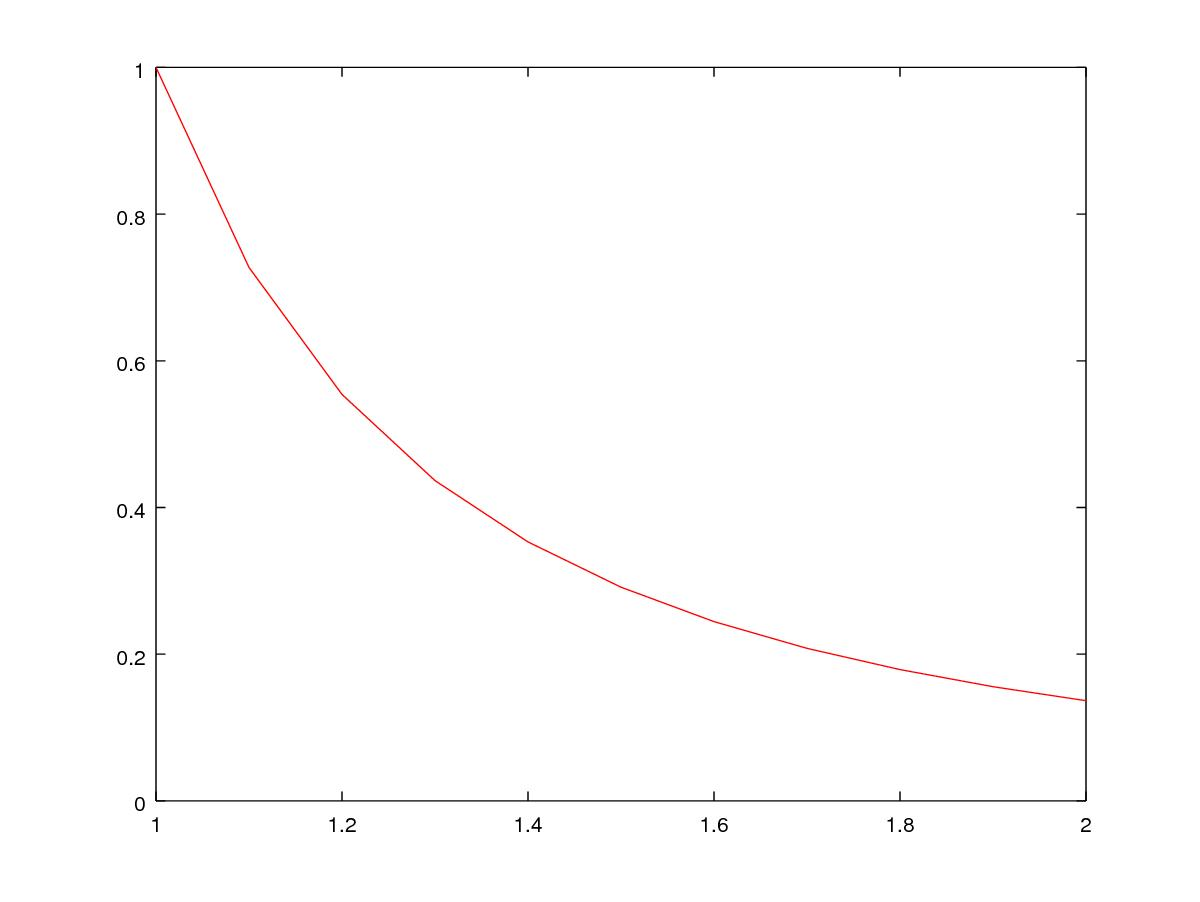
\includegraphics[width=\textwidth]{figs/metodo_eulero.jpg}
\caption{Grafico della soluzione con metodo di Eulero.}
\end{figure}
\end{center}

Possiamo confrontare la soluzione del metodo di Eulero con quella effettiva, data da $y(x)=\frac{1}{x^2(log(x)+1)}$,
con i seguenti comandi:

\begin{lstlisting}[frame=lines]
>> x=linspace(1,2,11);
>> real=@(x) 1./(x.^2.*(log(x)+1));
>> y=real(x);
>> hold on
>> plot(x,y,'b')
\end{lstlisting}
che ci restituiscono il seguente grafico:
\begin{center}
\begin{figure}[h!]
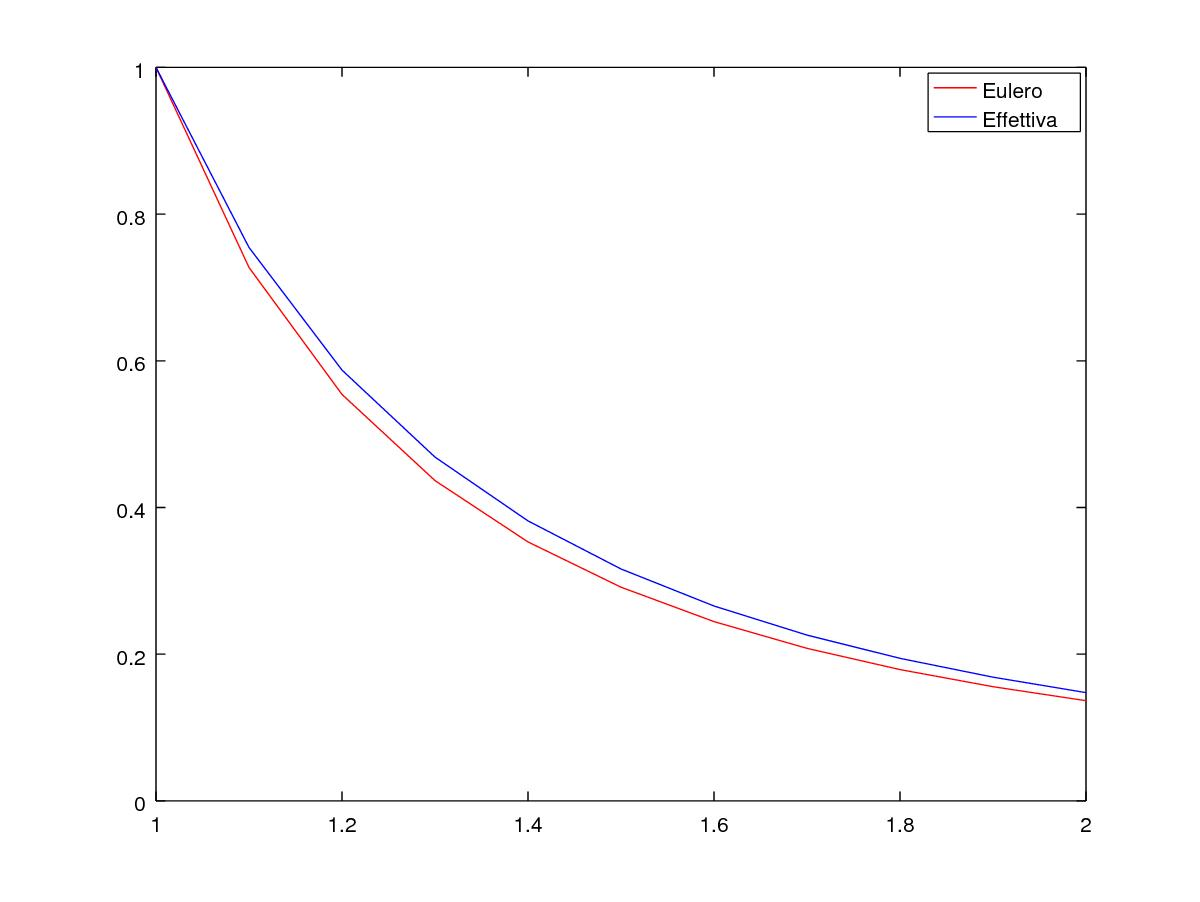
\includegraphics[width=0.60\textwidth]{figs/confronto_metodo_eulero.jpg}
\caption{Confronto delle soluzioni.}
\end{figure}
\end{center}


%SECONDO CAPITOLO
\chapter{Lezione II}
\section{Esercitazione II}
\subsection{Esercizio 1}
Per risolvere il problema test, usiamo lo script \emph{ese2\_1.m}:
\begin{lstlisting}[frame=trBL]
f=@(x,y) (-y);

subplot(2,2,1);
[x,u]=eulero(f, [0;10], 1, 0.5);
plot(x,u,'r');
hold on
plot(x,exp(-x),'b');
legend('metodo Eulero', 'soluzione esatta');
title('h=0.5');

subplot(2,2,2);
[x,u]=eulero(f, [0;10], 1, 1);
plot(x,u,'r');
hold on
plot(x,exp(-x),'b');
legend('metodo Eulero', 'soluzione esatta');
title('h=1');

subplot(2,2,3);
[x,u]=eulero(f, [0;10], 1, 2);
plot(x,u,'r');
hold on
plot(x,exp(-x),'b');
legend('metodo Eulero', 'soluzione esatta');
title('h=2');

subplot(2,2,4);
[x,u]=eulero(f, [0;10], 1, 2.5);
plot(x,u,'r');
hold on
plot(x,exp(-x),'b');
legend('metodo Eulero', 'soluzione esatta');
title('h=2.5');
\end{lstlisting}
dal quale otteniamo la seguente immagine:
\begin{figure}[h!]
\centering
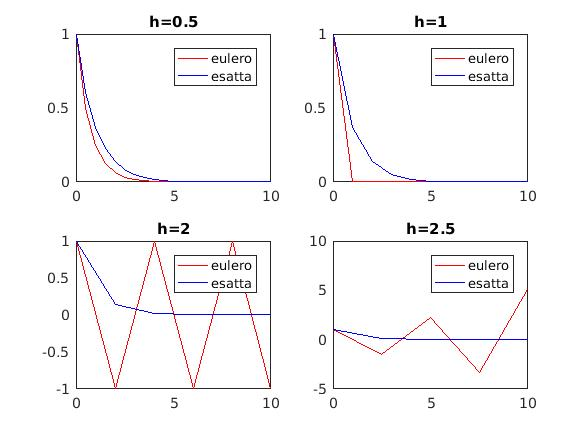
\includegraphics[width=\textwidth]{figs/ese2_1.jpg}
\end{figure}
\newpage

\subsection{Esercizio 2}
Implementazione del metodo di \textbf{Runge-Kutta classico}:
\begin{lstlisting}[frame=trBL]
function [x,u] = RK4(odefun,tspan,y0,h)
% Risolve sull'intervallo [tspan(1),tspan(2)] il problema :
%   y'(x) = odefun(x,y(x))
%   y(tspan(1)) = y0
% usando il metodo di Runge-Kutta classico
%
% Dati di INPUT:
%   odefun    funzione da integrare inizializzata VETTORIALMENTE
%   tspan     intervallo di integrazione
%   y0        condizione iniziale PER COLONNA
%   h         passo di discretizzazione
%
% Dati di OUTPUT:
%   x       nodi equispaziati della griglia
%   u       soluzione numerica in corrispondenza dei nodi

x = [tspan(1):h:tspan(2)];
N = length(x);
ord = length(y0);
u = zeros(ord, N);  
u(:, 1) = y0;
for i = 2:N
    f(:, 1) = odefun(x(i-1),u(:, i-1));
    f(:, 2) = odefun(x(i-1)+h/2,u(:, i-1)+h*f(:, 1)/2);
    f(:, 3) = odefun(x(i-1)+h/2, u(:, i-1)+h*f(:, 2)/2);
    f(:, 4) = odefun(x(i-1)+h, u(:, i-1)+h*f(:, 3));
    u(:, i) = u(:, i-1)+h/6*(f(:, 1)+2*f(:, 2)+2*f(:, 3)+f(:, 4));
end
end
\end{lstlisting}
Per risolvere quindi il problema dato, definiamo la funzione \emph{fun2\_2.m}:
\begin{lstlisting}[frame = lines]
function f=fun2_2(x, y)
f(1) = y(2);
f(2) = ((-(4*x+1)/(2*x+2))*y(2)+(2*x-1)*(3*y(1)^3+y(1)))/...
            ((4*x^2)*(1+y(1)^2));
end
\end{lstlisting}
e risolviamo infine il problema con lo script \emph{ese2\_2.m}:
\begin{lstlisting}[frame=trBL]
[x,u] = RK4(@(x, y) fun2_2(x, y),[1;2],[1;0],0.01);
plot(x, u(1, :), 'r');
hold on
plot(x, u(2, :), 'b');
legend('y(x)', 'dy(x)/dx');
\end{lstlisting}
dal quale otteniamo il grafico delle soluzioni:
\begin{figure}[h!]
\centering
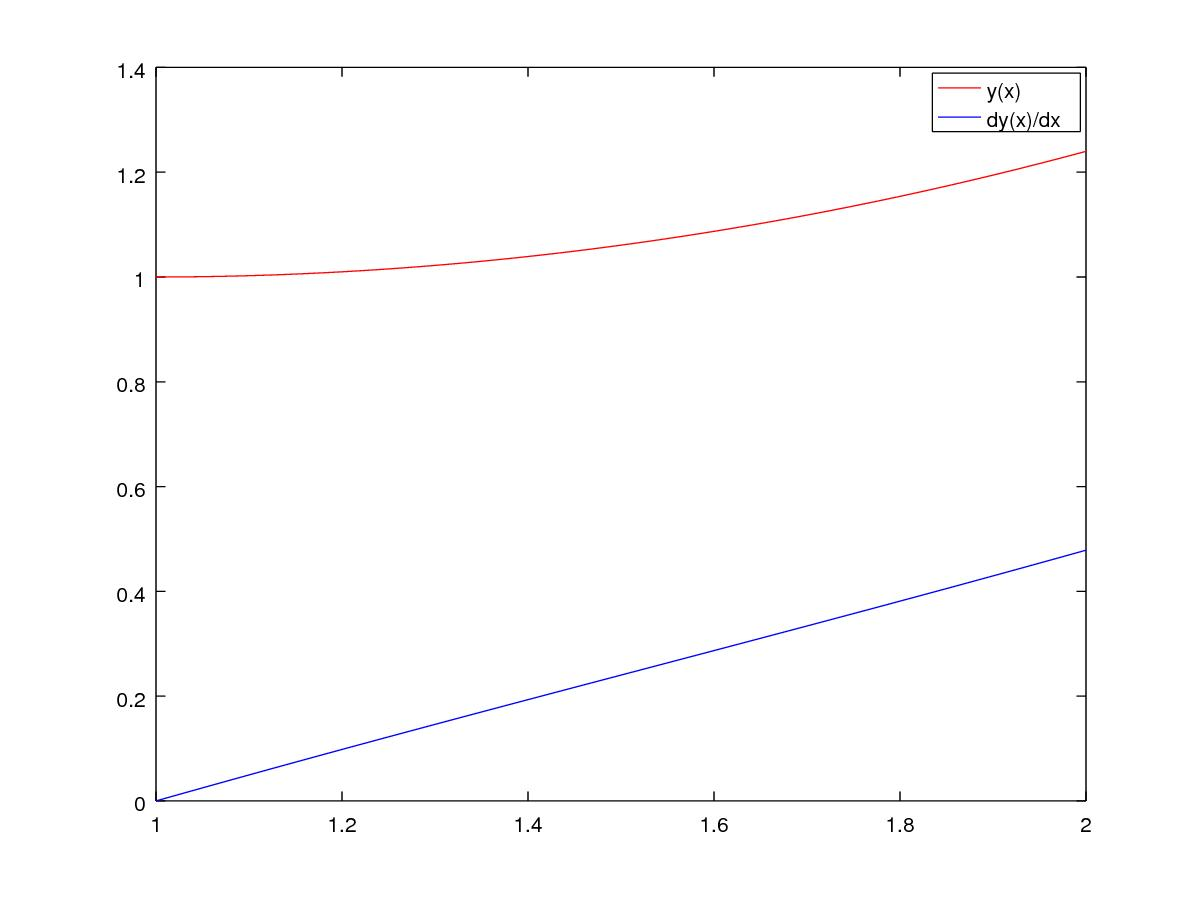
\includegraphics[width=\textwidth]{figs/ese2_2.jpg}
\end{figure}

\newpage
\subsection{Esercizio 3}
Per risolvere l'esercizio 3, per prima cosa definisco la funzione \emph{fun2\_3.m}:
\begin{lstlisting}[frame=trBL]
function f=fun2_3(t, y)
f = -y-5*exp(-t)*sin(5*t);
end
\end{lstlisting}

Successivamente, creo lo sript \emph{ese2\_3.m}:
\begin{lstlisting}[frame=trBL]
f=@(t, y) fun2_3(t, y);
tspan = [0,5];
init = 1;
esatta = @(t) (exp(-t)*cos(5*t));
A = zeros(10, 3);
for i=1:10
    A(i, 1) = 0.1/(2^(i-1));
    [x, u] = eulero(f, tspan, init, A(i, 1));
    A(i, 2) = abs(u(find(x==2))-esatta(2));
    [x, u] = RK4(f, tspan, init, A(i, 1));
    A(i, 3) = abs(u(find(x==2))-esatta(2));
end
\end{lstlisting}
Nella matrice $A$ salviamo, nella seconda e terza colonna, rispettivamente le differenze dalla soluzione esatta
sia del metodo di Eulero che del metodo di Runge-Kutta.
\begin{lstlisting}[frame = lines]
>> A(:, 2:end)
ans =

   4.01861453386227e-02   4.85009807628389e-06
   2.06896235879312e-02   2.99815263934966e-07
   1.04924790909868e-02   1.86718078776238e-08
   5.28307689880908e-03   1.16546573780685e-09
   2.65074396138568e-03   7.28026250396141e-11
   1.32767325159178e-03   4.54905557667473e-12
   6.64411953038790e-04   2.84133827577193e-13
   3.32349810943169e-04   1.81799020282369e-14
   1.66210864492380e-04   1.36002320516582e-15
   8.31144220587998e-05   8.04911692853238e-16
\end{lstlisting}
Per stimare l'ordine di convergenza dei due metodi basterà calcolare i valori $log_{2}(\frac{A(j,2)}{A(j+1,2)})$ e 
$log_{2}(\frac{A(j,3)}{A(j+1,3)})$ per $j=1, 2, \dots, 9$. Per eseguire questi calcoli usiamo lo script \emph{stima\_ord}:
\begin{lstlisting}[frame = trBL]
function [O]=stima_ord(A)
[n, m]=size(A);
O = zeros(n-1, 2);

for j=1:n-1
    O(j,1)=log2(A(j,2)/A(j+1,2));
    O(j,2)=log2(A(j,3)/A(j+1,3));
end
end
\end{lstlisting}
Eseguendolo sulla matrice $A$ di prima, otteniamo la seguente tabella:
\begin{lstlisting}[frame = lines]
>> stima_ord(A)
ans =

   0.957790802412968   4.015868181551954
   0.979551809806176   4.005140307567236
   0.989905273706966   4.001883123652946
   0.994981084210094   4.000772312199786
   0.997497190846278   4.000351504996218
   0.998750201091335   4.000924553369065
   0.999375494978621   3.966154271973940
   0.999687845233656   3.740641252309604
   0.999843946944397   0.756728848987636

\end{lstlisting}
Dai dati di questa tabella si capisce che l'ordine di convergenza del metodo di Eulero è 1, mentre l'ordine
del metodo di Runge-Kutta è 4. (L'ultimo valore della seconda colonna credo sia dovuto al fatto che l'ultimo elemento 
della terza colonna di $A$ sia molto vicino alla precisione di macchina.) %
\footnote{$eps = 2.22044604925031e-16$}



\newpage
\subsection{Esercizio 4}
Per risolvere il punto (a) usiamo lo script \emph{ese2\_4\_a.m}:
\begin{lstlisting}[frame=trBL]
f = @(x, y) ((2*y)/x)+(x^2)*exp(x);
g = @(x) (x.^2).*(exp(x) - exp(1));
slot = [1, 2];
init = 0;

subplot(2,2,1)
[x, u]=eulero(f, slot, init, 0.5);
[x1, u1] = ode45(f, slot, init);
plot(x, u, 'r')
hold on
plot(x, g(x), 'g');
hold on
plot(x1, u1, 'b');
legend('Eulero', 'Sol. Esatta', 'Ode45');
title('h=0.5');

subplot(2,2,2)
[x, u]=eulero(f, slot, init, 1);
[x1, u1] = ode45(f, slot, init);
plot(x, u, 'r')
hold on
plot(x, g(x), 'g');
hold on
plot(x1, u1, 'b');
legend('Eulero', 'Sol. Esatta', 'Ode45');
title('h=1');

subplot(2,2,3)
[x, u]=eulero(f, slot, init, 0.7);
[x1, u1] = ode45(f, slot, init);
plot(x, u, 'r')
hold on
plot(x, g(x), 'g');
hold on
plot(x1, u1, 'b');
legend('Eulero', 'Sol. Esatta', 'Ode45');
title('h=0.7');

subplot(2,2,4)
[x, u]=eulero(f, slot, init, 0.1);
[x1, u1] = ode45(f, slot, init);
plot(x, u, 'r')
hold on
plot(x, g(x), 'g');
hold on
plot(x1, u1, 'b');
legend('Eulero', 'Sol. Esatta', 'Ode45');
title('h=0.1');
\end{lstlisting}

che ci restituisce la seguente immagine:
\begin{figure}[h!]
\centering
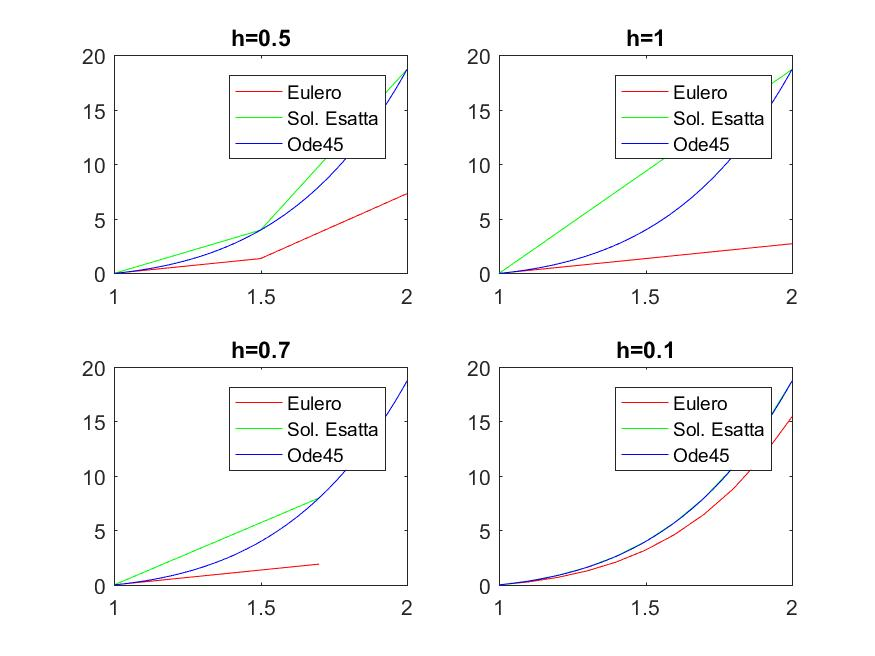
\includegraphics[width=\textwidth]{figs/ese2_4_a.jpg}
\caption{Sistema a.}
\end{figure}
\par
Utilizzando degli script analoghi, in cui le uniche differenze stanno nella funzione e nei
valori di slot e init, si ottengono le seguenti 2 immagini:
\begin{figure}[h!]
\centering
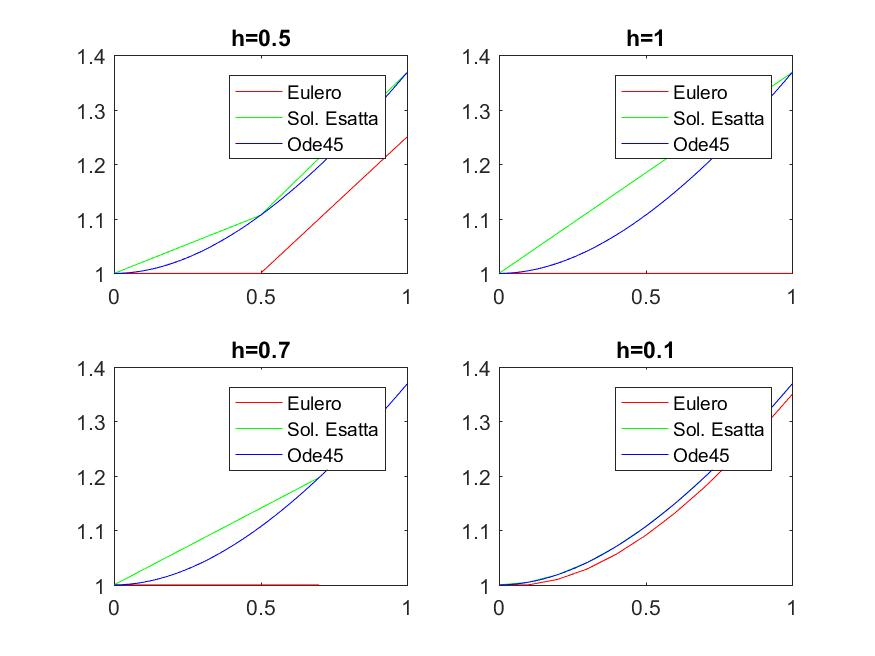
\includegraphics[width=\textwidth]{figs/ese2_4_b.jpg}
\caption{Sistema b.}
\end{figure}

\begin{figure}[t!]
\centering
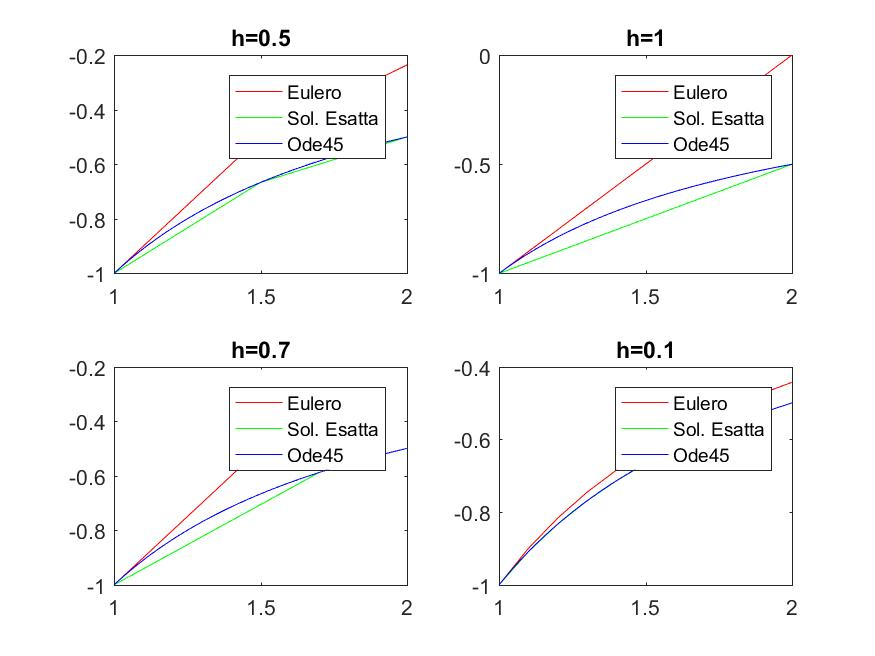
\includegraphics[width=\textwidth]{figs/ese2_4_c.jpg}
\caption{Sistema c.}
\end{figure}

\newpage
\subsection{Esercizio 5}
Per risolvere l'esercizio 5, usiamo lo script \emph{ese2\_5.m}:
\begin{lstlisting}[frame=trBL]
function ese2_5(a)
f=@(x, y) -a*y+2*x;
g=@(x) (1-(2/a^2))*exp(-a.*x)+(2/a).*x-2/a^2;
slot=[0, 6];
init = 1;

[x, u]=eulero(f, slot, init, 0.1);
[a,b]=ode45(f, slot, init);
err_a_Eulero_1=abs(u'-g(x));
err_rel_Eulero_1=[0, abs(g(x(2:end))-(g(x(1:end-1))+...
            (0.1)*f(x(1:end-1),g(x(1:end-1)))))];

[x1, u1]=eulero(f, slot, init, 0.01);
[a,b]=ode45(f, slot, init);
err_a_Eulero_2=abs(u1'-g(x1));
err_rel_Eulero_2=[0, abs(g(x1(2:end))-(g(x1(1:end-1))+...
            (0.1)*f(x1(1:end-1),g(x1(1:end-1)))))];

[x2, u2]=eulero(f, slot, init, 0.001);
[a,b]=ode45(f, slot, init);
err_a_Eulero_3=abs(u2'-g(x2));
err_rel_Eulero_3=[0, abs(g(x2(2:end))-(g(x2(1:end-1))+...
            (0.1)*f(x2(1:end-1),g(x2(1:end-1)))))];

options = odeset('RelTol', 10^(-7));
[v, w]=ode45(f, slot, init, 'options');
err_a_ode=abs(w-g(v));
step=v(2:end)-v(1:end-1);

figure
hold on
plot(x, err_a_Eulero_1, 'r');
plot(x1, err_a_Eulero_2, 'b');
plot(x2, err_a_Eulero_3, 'y');
plot(v, err_a_ode, 'g');
legend('h=0.1', 'h=0.01', 'h=0.001', 'ode');
title('Errori Assoluti');

figure
hold on
plot(x, err_rel_Eulero_1, 'r');
plot(x1, err_rel_Eulero_2, 'b');
plot(x2, err_rel_Eulero_3, 'y');
legend('h=0.1', 'h=0.01', 'h=0.001');
title('Errori Relativi');

figure 
hold on
plot(step, 'r');
title('Passo di Integrazione');

figure
hold on
plot(x,u,'b');
plot(x1, u1, 'g');
plot(x2, u2, 'r');
plot(v, w, 'y');
legend('h=0.1', 'h=0.01', 'h=0.001', 'ode');
title('soluzioni');

end
\end{lstlisting}
\newpage
Lanciandolo con $a=1$, si ottengono le seguenti 4 immagini:
\begin{figure}[h!]
\centering
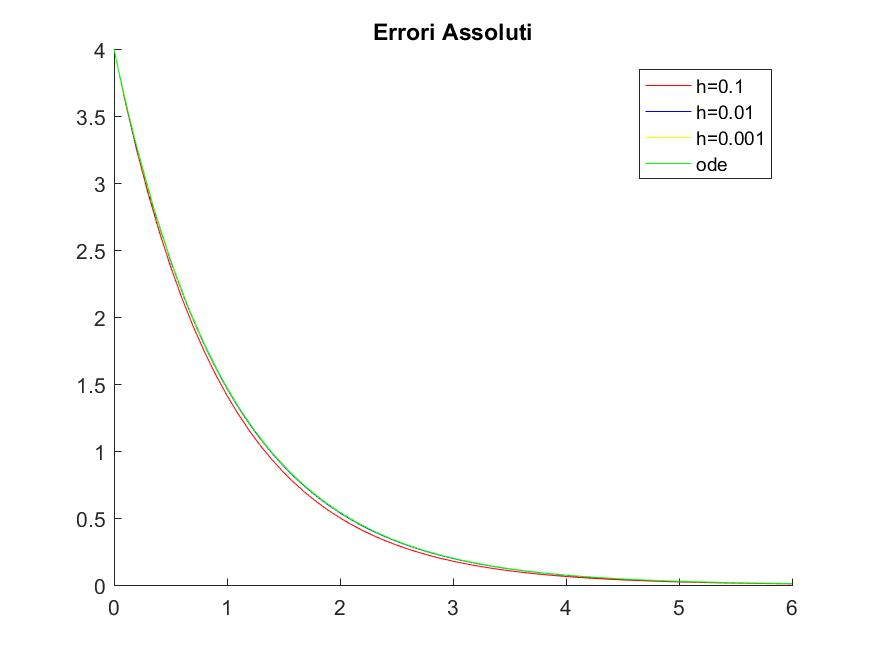
\includegraphics[width=\textwidth]{figs/errori_assoluti_1.jpg}
\caption{$a=1$}
\end{figure}
\begin{figure}[h!]
\centering
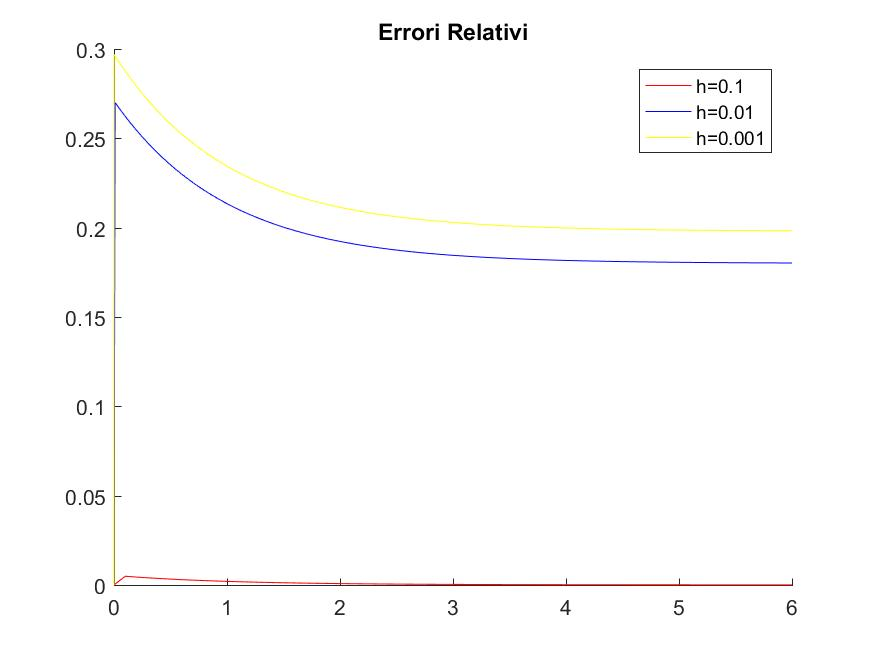
\includegraphics[width=\textwidth]{figs/errori_relativi_1.jpg}
\caption{$a=1$}
\end{figure}
\begin{figure}[h!]
\centering
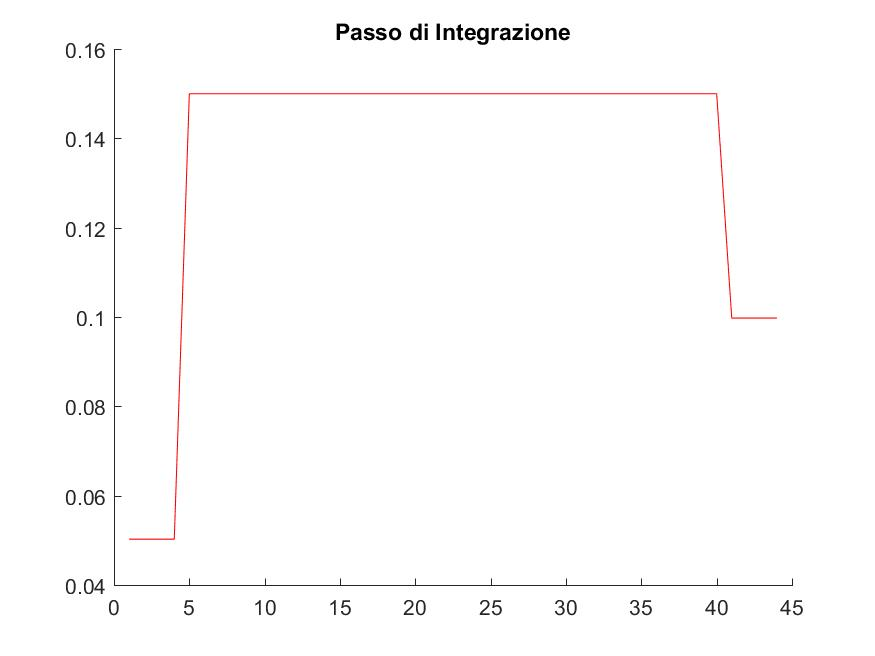
\includegraphics[width=\textwidth]{figs/step_ode_1.jpg}
\caption{$a=1$}
\end{figure}
\begin{figure}[h!]
\centering
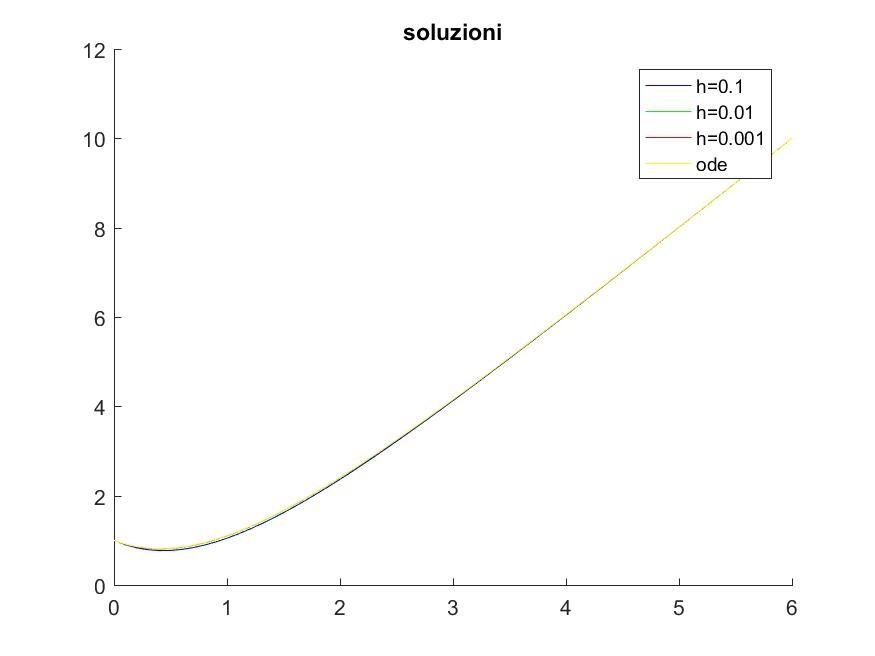
\includegraphics[width=\textwidth]{figs/soluzioni_1.jpg}
\caption{$a=1$}
\end{figure}


\newpage
Lanciandolo con $a=100$, si ottengono invece le seguenti immagini:
\begin{figure}[h!]
\centering
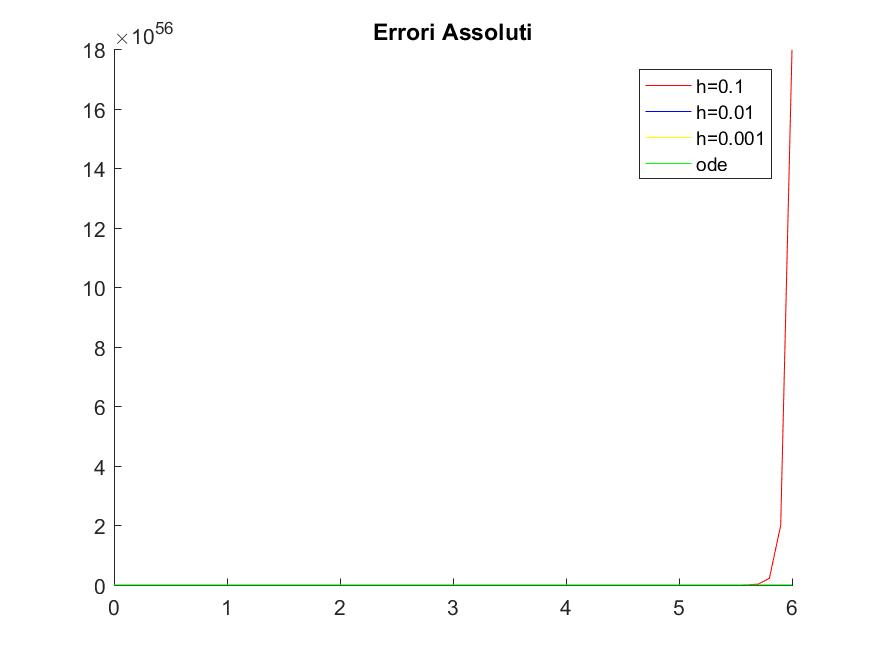
\includegraphics[width=\textwidth]{figs/errori_assoluti_100.jpg}
\caption{$a=100$}
\end{figure}
\begin{figure}[h!]
\centering
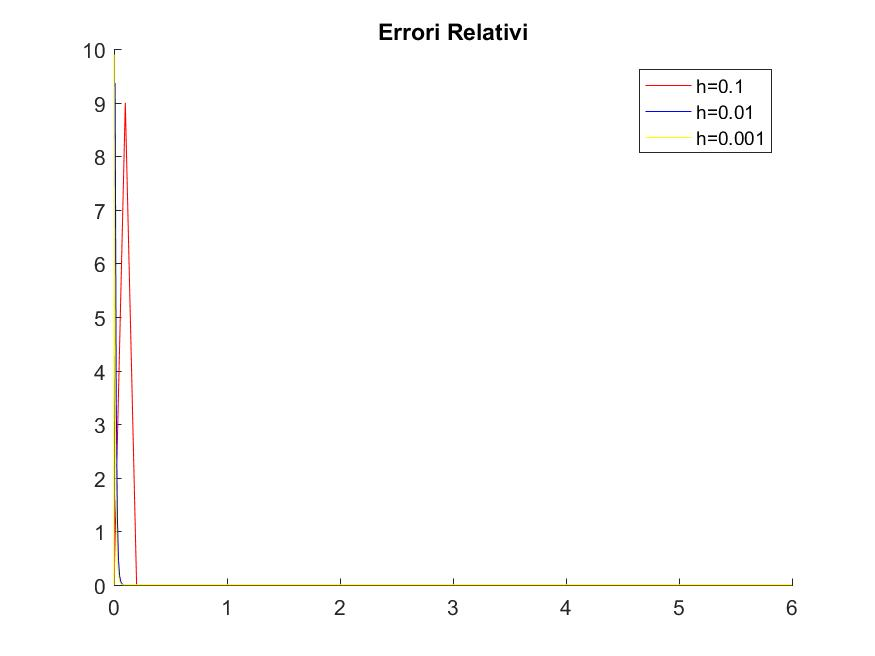
\includegraphics[width=\textwidth]{figs/errori_relativi_100.jpg}
\caption{$a=100$}
\end{figure}
\begin{figure}[h!]
\centering
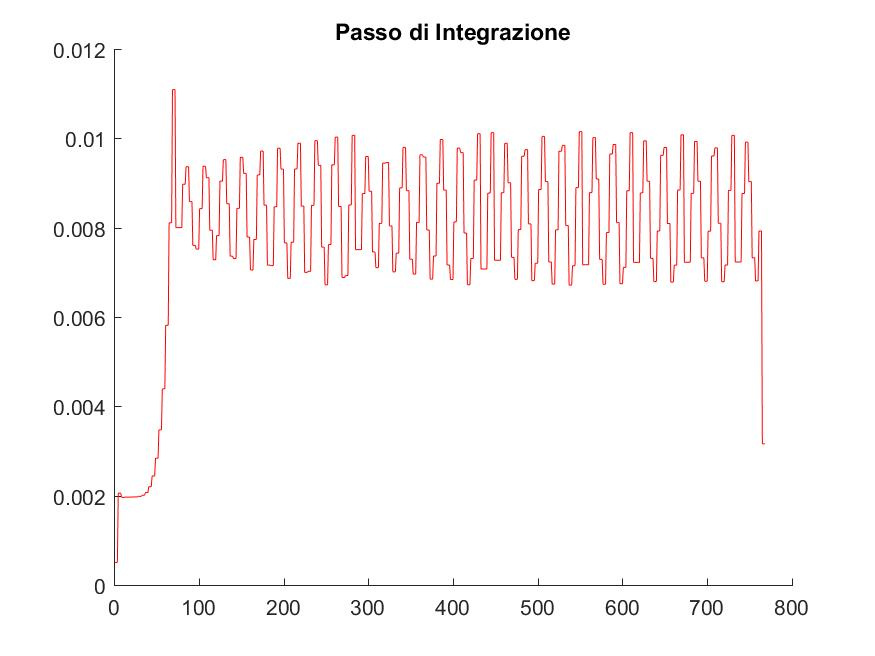
\includegraphics[width=\textwidth]{figs/step_ode_100.jpg}
\caption{$a=100$}
\end{figure}
\begin{figure}[h!]
\centering
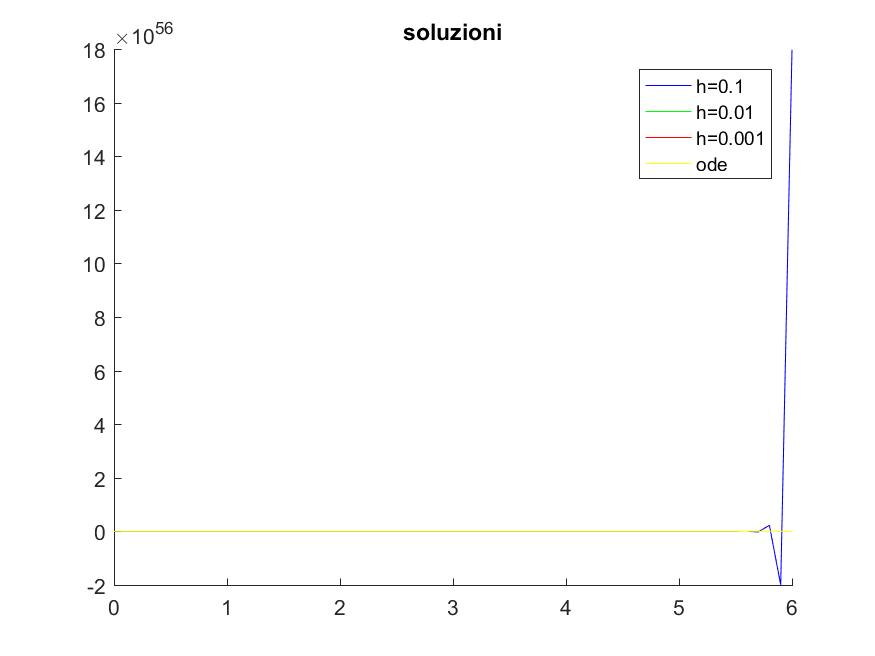
\includegraphics[width=\textwidth]{figs/soluzioni_100.jpg}
\caption{$a=100$}
\end{figure}




%TERZO CAPITOLO
\chapter{Lezione III}
\section{Esercitazione III}
\subsection{Esercizio 1}
La function \emph{ese1\_s.m}:
\begin{lstlisting}[frame=trBL]
function ese1_s 

slot=[0,6];
h=0.1;
init=1000;
odefun=@(x,y)(log(2)*y);
[x,u] = eulero(odefun,slot,init,h);
plot(x,u,'r')
\end{lstlisting}
dalla quale otteniamo la seguente figura:
\begin{center}
\begin{figure}[h!]
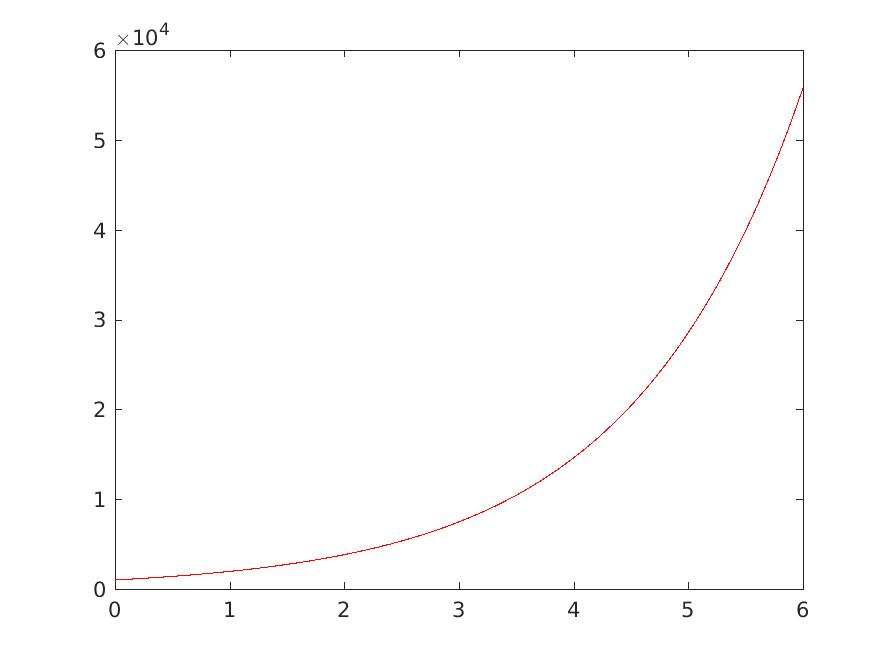
\includegraphics[width=\textwidth]{figs/ese1_s.jpg}
\caption{Numero di batteri presenti nelle prime 6 ore.}
\end{figure}
\end{center}

\subsection{Esercizio 2}
L'esercizio 2 si risolve con il seguente script:
\begin{lstlisting}[frame=trBL]
f=@(x,y)(-log(2)*y/50);
y0=1;
h=1;
tspan=[0, 200];
[x,u]=RK4(f,tspan,y0,h);
plot(x,u,'r');
y=find(u<=0.1);
x(y(1))
hold on
plot(x(y(1)), u(y(1)), '*b'); 
\end{lstlisting}
dal quale otteniamo la seguente immagine:
\begin{center}
\begin{figure}[h!]
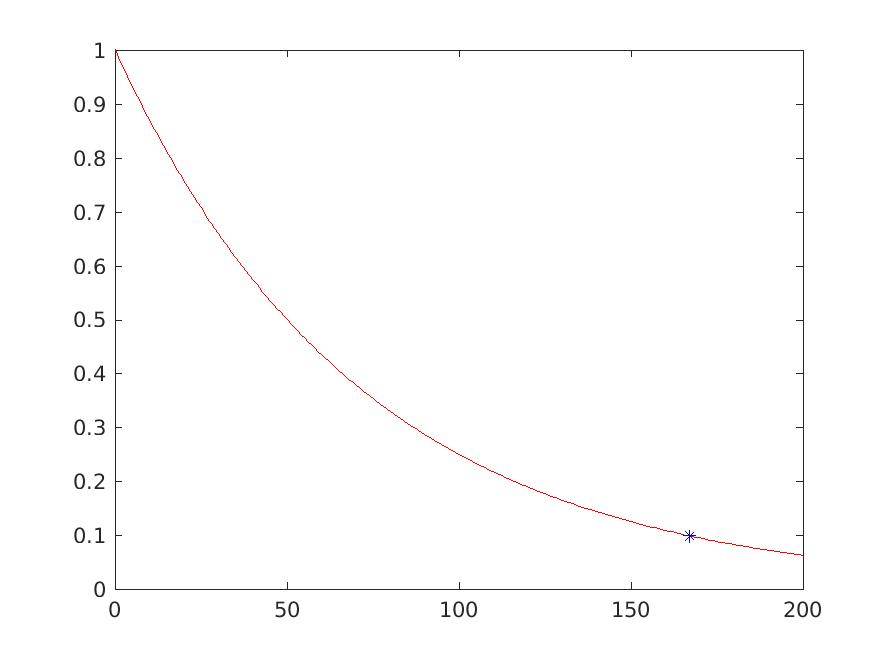
\includegraphics[width=\textwidth]{figs/ese2_s.jpg}
\caption{Quantità di plutonio presente nei primi 200 anni.}
\end{figure}
\end{center}
L'asterisco indica quando la quantità di plutonio è $\frac{1}{10}$ di quella iniziale.
\subsection{Esercizio 3}
Lo script \emph{ese3\_s.m} è:
\begin{lstlisting}[frame=trBL]
f=@(x,y)(0.2*y*(1-(y/0.01)));
[x,u]=ode45(f,[0,0.5], 2);
plot(x,u, 'r');
hold on
z=find(u<=0.2);
plot(x(z(1)),u(z(1)), '*b');
\end{lstlisting}
dal quale si ottiene la seguente immagine:
\begin{center}
\begin{figure}[h!]
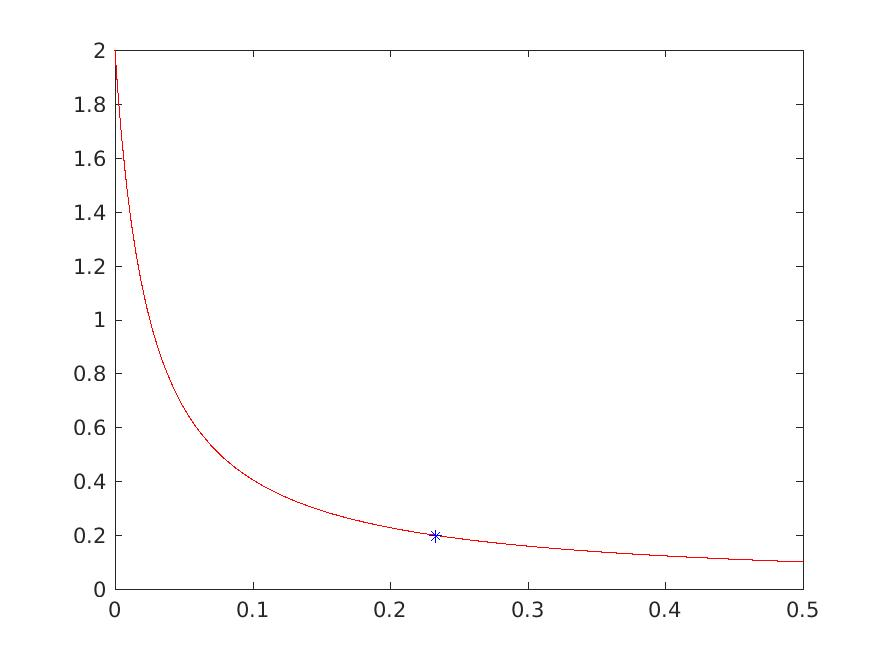
\includegraphics[width=\textwidth]{figs/ese3_s.jpg}
\caption{Grafico della densità di popolazione.}
\end{figure}
\end{center}
L'asterisco indica in quale istante la densità di popolazione è 
$\frac{1}{10}$ di quella iniziale.
\subsection{Esercizio 4}
L'esercizio 4 si risolve con il seguente script:
\begin{lstlisting}[frame=trBL]
alpha=@(t)(1/2+cos(2*pi*t));
f=@(t,y)(alpha(t)*y*(1-y/100));
slot=[0,20];
y0=[1,10,50,200];
for i=1:4
    [x,u]=ode45(f, slot, y0(i));
    subplot(2,2,i);
    plot(x,u,'r');
    title(y0(i));
end
\end{lstlisting}
dal quale otteniamo le seguenti immagini:
\begin{center}
\begin{figure}[h!]
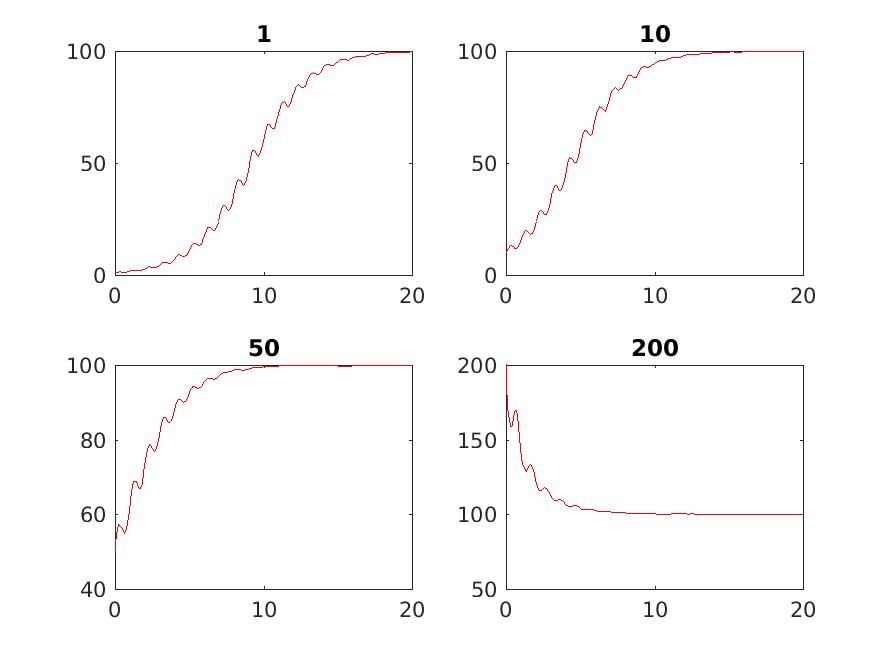
\includegraphics[width=\textwidth]{figs/ese4_s.jpg}
\caption{Grafico dell'equazione $y(t)$ per i valori $y_{0}=1,10,50,200$.}
\end{figure}
\end{center}

\newpage
\section{Esercitazione IV}
\subsection{Esercizio 1}
Per risolvere il modello di Lotka-Volterra con i parametri determinati da Gause, 
usiamo lo script \emph{odefun1.m}:
\begin{lstlisting}[frame=trBL]
g1=0.21827;
k1=13;
h1=3.71429;
g2=0.06069;
k2=5.8;
h2=13.2118;
f=zeros(2, 1);
f=@(t, y) [g1*(1-y(1)/k1-y(2)/h1)*y(1);g2*(1-y(2)/k2-y(1)/h2)*y(2)];
slot = [0, 300];
init = [0.5;0.3];
[t, u]=ode45(f, slot, init);
hold on
plot(t, u(:,1), 'r');
plot(t, u(:,2), 'b');
legend('Saccharomyces cerevisiae', 'Schizosaccharomyces kephir');
\end{lstlisting}
dal quale otteniamo la seguente immagine:
\begin{center}
\begin{figure}[h!]
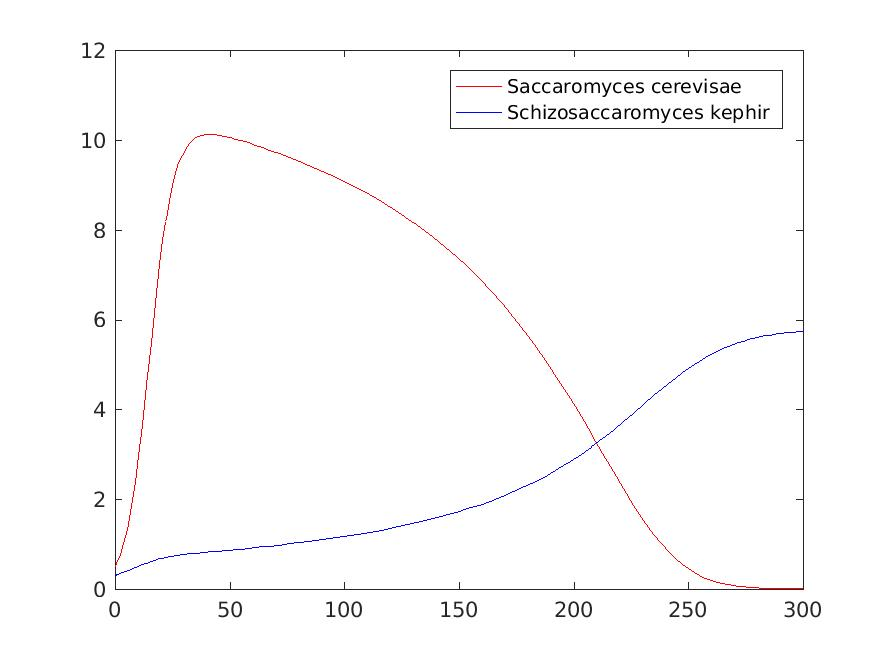
\includegraphics[width=\textwidth]{figs/paolomyces.jpg}
\caption{Densità di popolazione dei due batteri.}
\end{figure}
\end{center}
\newpage
Modifichiamo lo script \emph{odefun1.m} per ottenere lo script
\emph{odefun1\_bis.m} che risolve il resto del problema:
\begin{lstlisting}[frame=trBL]
g1=0.21827;
k1=13;
h1=3.71429;
g2=0.06069;
k2=5.8;
h2=13.2118;
f=zeros(2, 1);
f=@(t, y) [g1*(1-y(1)/k1-y(2)/h1)*y(1);g2*(1-y(2)/k2-y(1)/h2)*y(2)];
slot=[0, 300];
init1=[0.5; 0.5];
init2=[0.1; 0.5];
init3=[10;0.5];

subplot(3, 1, 1)
[t, u]=ode45(f, slot, init1);
hold on
plot(t, u(:,1), 'r');
plot(t, u(:,2), 'b');
legend('Saccharomyces cerevisiae', 'Schizosaccharomyces kephir');
title('N1(0)=0.5');

subplot(3, 1, 2)
[t, u]=ode45(f, slot, init2);
hold on
plot(t, u(:,1), 'r');
plot(t, u(:,2), 'b');
legend('Saccharomyces cerevisiae', 'Schizosaccharomyces kephir');
title('N1(0)=0.1');

subplot(3, 1, 3)
[t, u]=ode45(f, slot, init3);
hold on
plot(t, u(:,1), 'r');
plot(t, u(:,2), 'b');
legend('Saccharomyces cerevisiae', 'Schizosaccharomyces kephir');
title('N1(0)=10');
\end{lstlisting}
dal quale otteniamo le seguenti immagini:
\begin{center}
\begin{figure}[h!]
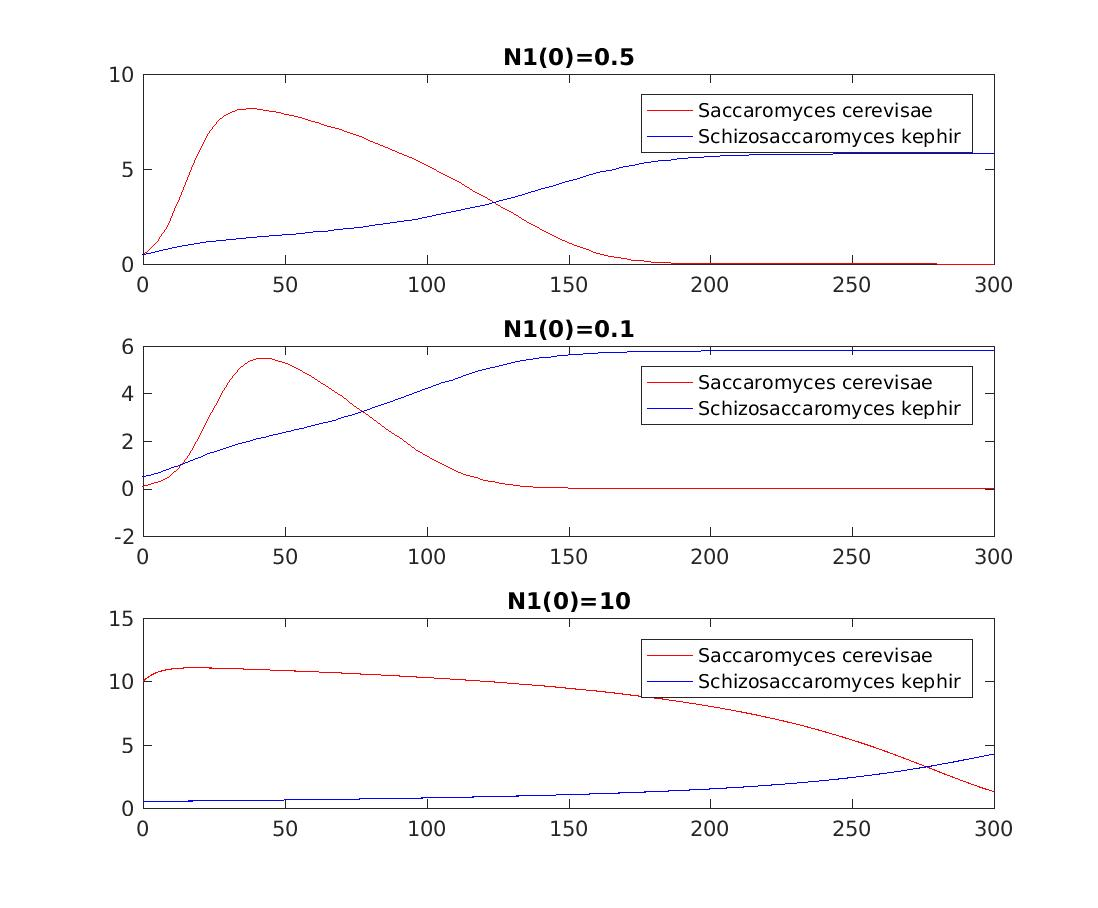
\includegraphics[width=\textwidth]{figs/diegomyces.jpg}
\caption{Densità delle popolazioni al variare di N1(0).}
\end{figure}
\end{center}

\subsection{Esercizio 2}
Per risolvere questo esercizio usiamo lo script \emph{odefun2.m}:
\begin{lstlisting}[frame=trBL]
a=2;
b=0;
g=0.001;
a1=1;
b1=0.001;
f=@(t, y) [(a-b*y(1)-g*y(2))*y(1);(-a1+b1*y(1))*y(2)];
slot=[0, 5];
init1=[300;150];
init2=[15;22];

figure;
[t, u]=RK4(f, slot, init1, 0.01);
hold on
plot(t, u(1,:), 'r');
plot(t, u(2,:), 'b');
legend('preda', 'predatore');
title('preda(0)=300, predatore(0)=150');
figure;
plot(u(1,:), u(2,:), 'g');
title('predatori rispetto alle prede');



figure;
[t, u]=RK4(f, slot, init2, 0.01);
hold on
plot(t, u(1,:), 'r');
plot(t, u(2,:), 'b');
legend('preda', 'predatore');
title('preda(0)=15, predatore(0)=22');
figure;
plot(u(1,:), u(2,:), 'g');
title('predatori rispetto alle prede');
\end{lstlisting}
Da questo script si ottengono queste immagini:
\begin{center}
\begin{figure}[h!]
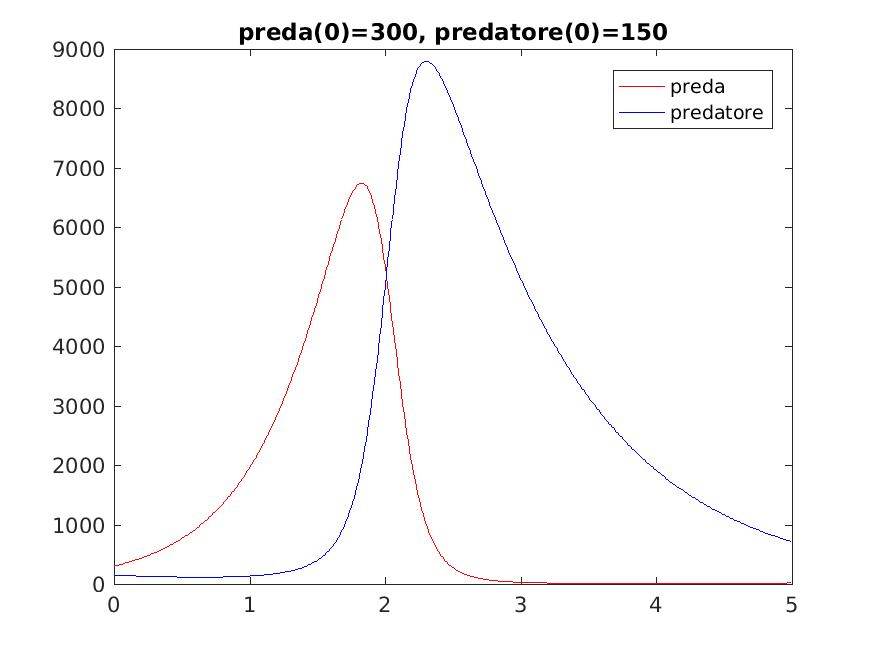
\includegraphics[width=\textwidth]{figs/preda.jpg}
\caption{Soluzioni relative alle prede ed ai predatori con init=[300;150].}
\end{figure}
\end{center}
\begin{center}
\begin{figure}[h!]
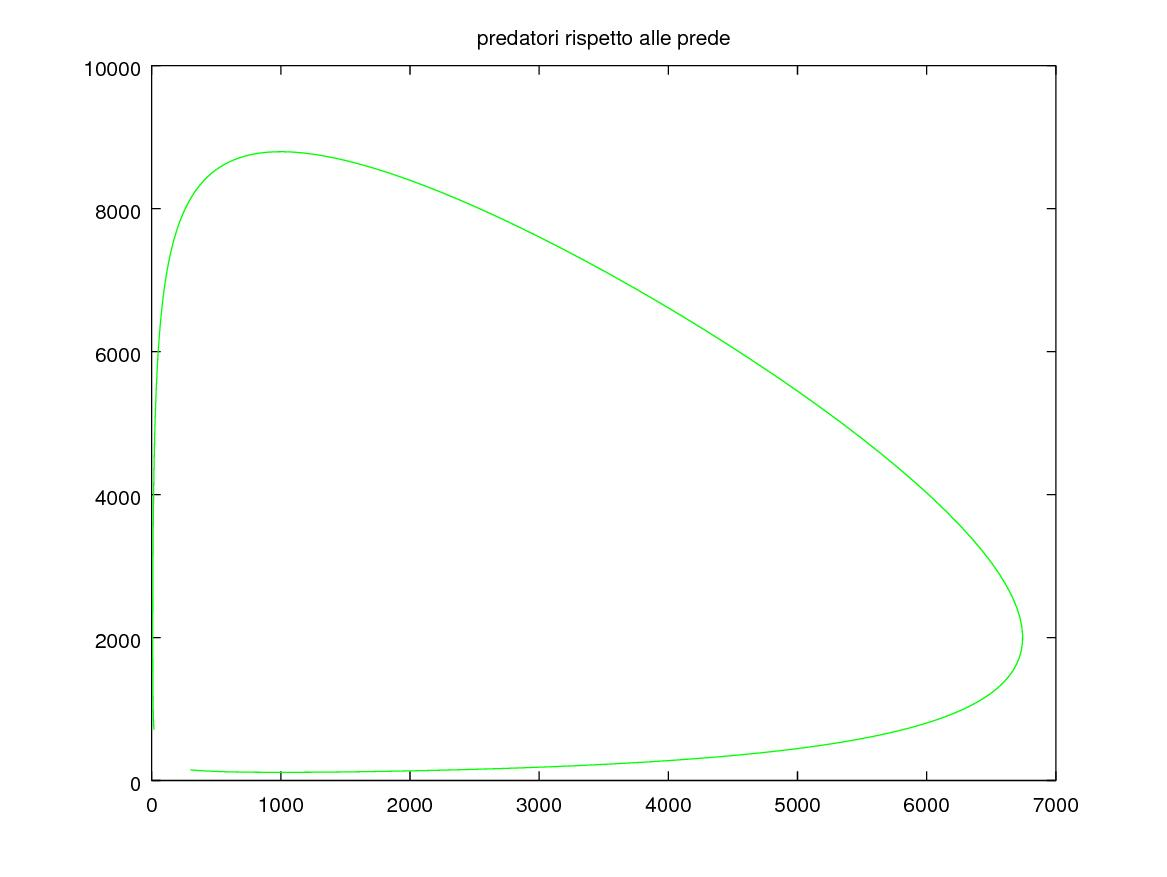
\includegraphics[width=\textwidth]{figs/predatore_preda.jpg}
\caption{Preda rispetto al predatore con init=[300;150].}
\end{figure}
\end{center}
\begin{center}
\begin{figure}[h!]
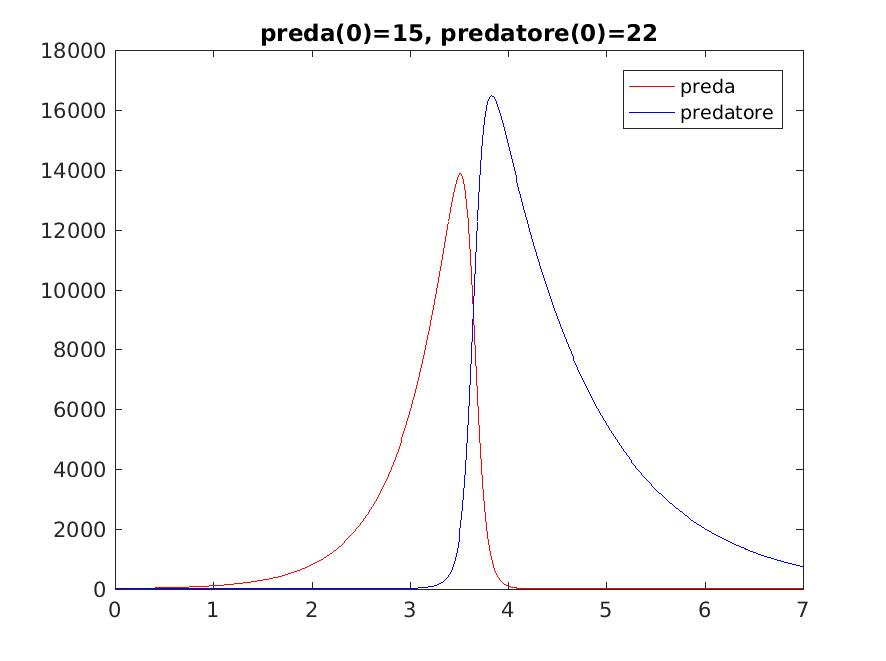
\includegraphics[width=\textwidth]{figs/preda15.jpg}
\caption{Soluzioni relative alle prede ed ai predatori con init=[15;22].}
\end{figure}
\end{center}
\begin{center}
\begin{figure}[t!]
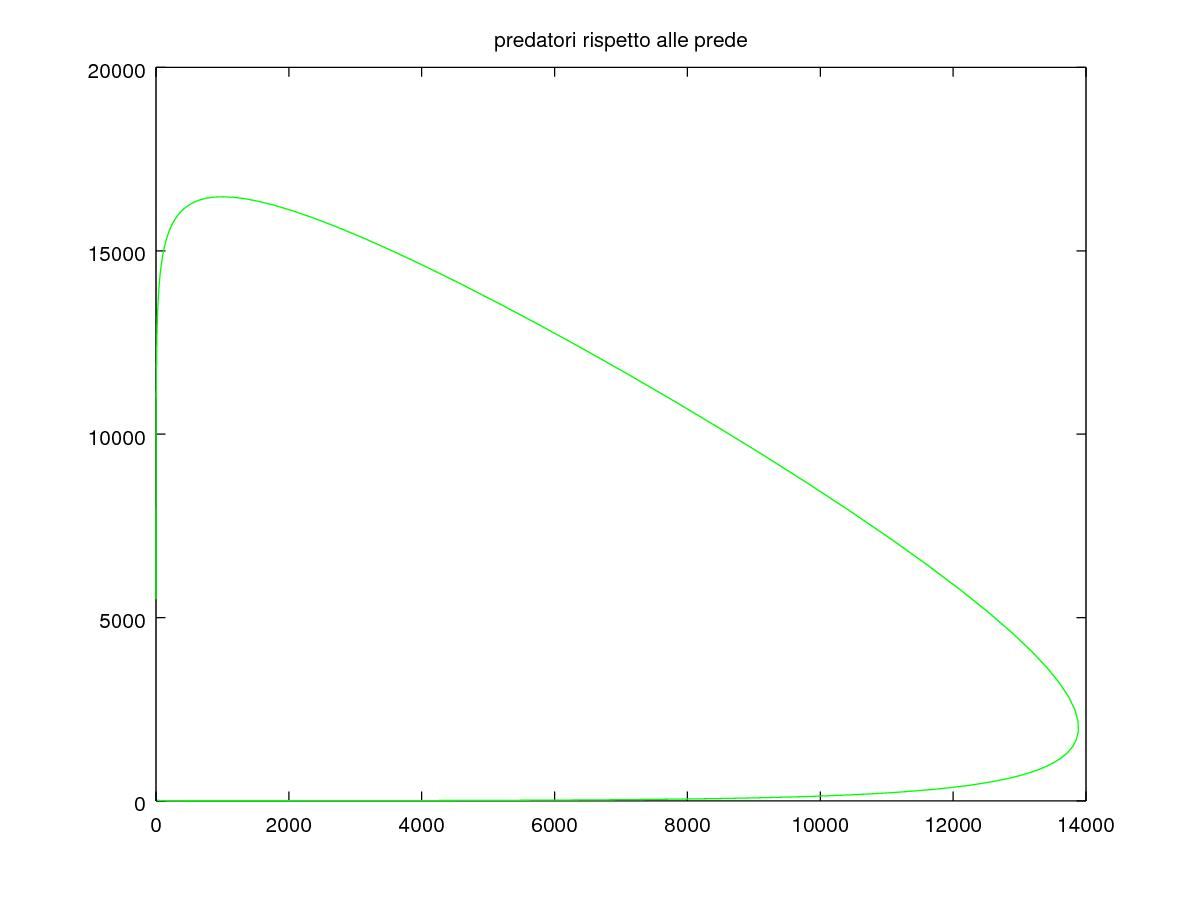
\includegraphics[width=\textwidth]{figs/predatore_preda_15.jpg}
\caption{Preda rispetto al predatore con init=[15;22].}
\end{figure}
\end{center}

\newpage
\subsection{Esercizio 3}
Risolviamo l'esercizio 3 con lo script \emph{odefun3.m}:
\begin{lstlisting}[frame = trBL]
f=@(t, y) [0.405*y(1)-0.81*y(1)*y(2); -1.5*y(2)+0.125*y(1)*y(2)];

[t, u]= ode45(f, [0, 10], [7.7; 0.5]);
plot(u(:,1), u(:,2), 'b');
title('Predatori in funzione delle prede con T=10');

figure
hold on
[t, u]= ode45(f, [0, 25], [7.7; 0.5]);
plot(t, u(:,1), 'r');
plot(t, u(:,2), 'b');
legend('prede', 'predatori');
title('Prede e predatori con T=25');
\end{lstlisting}
Le immagini che otteniamo sono:
\begin{center}
\begin{figure}[h!]
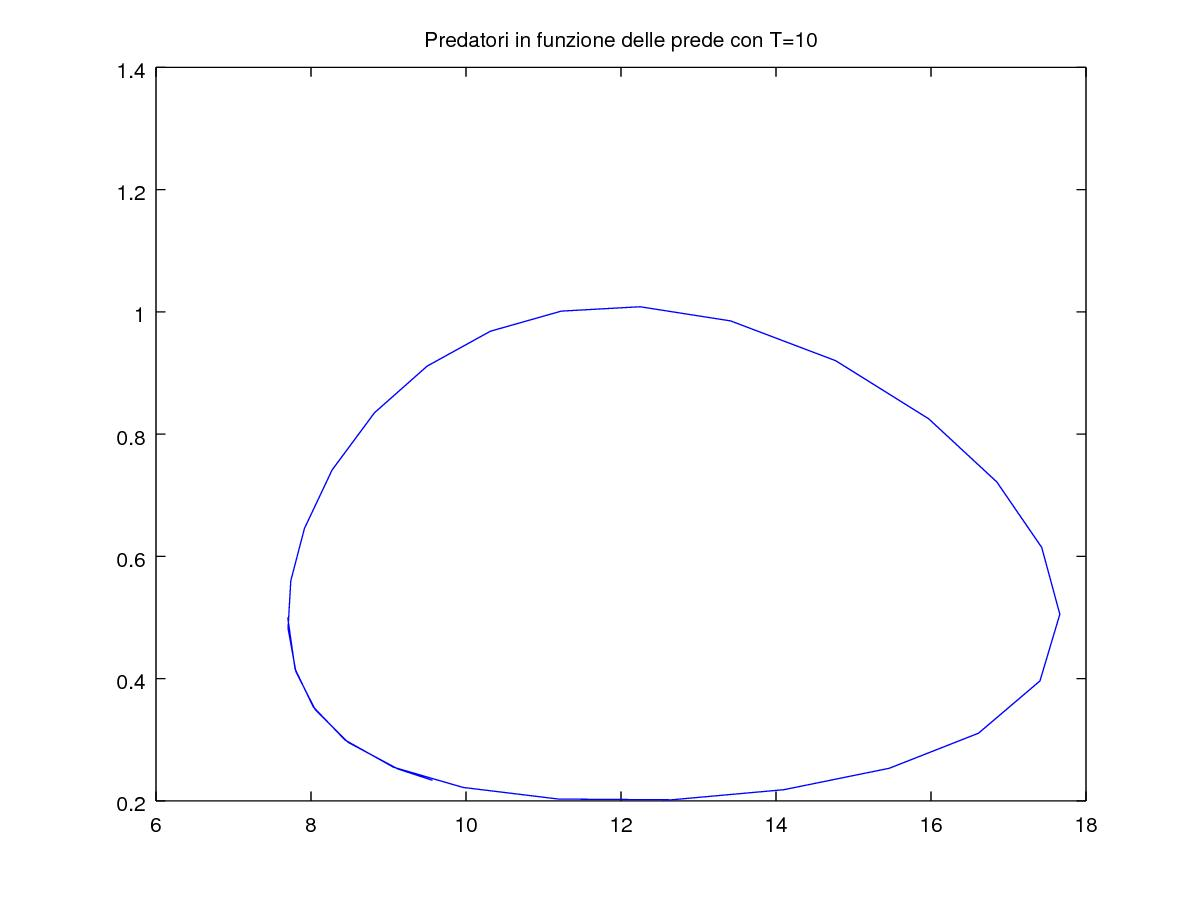
\includegraphics[width=\textwidth]{figs/predatori_prede_10.jpg}
\caption{Preda rispetto al predatore con T=10.}
\end{figure}
\end{center}

\begin{center}
\begin{figure}[h!]
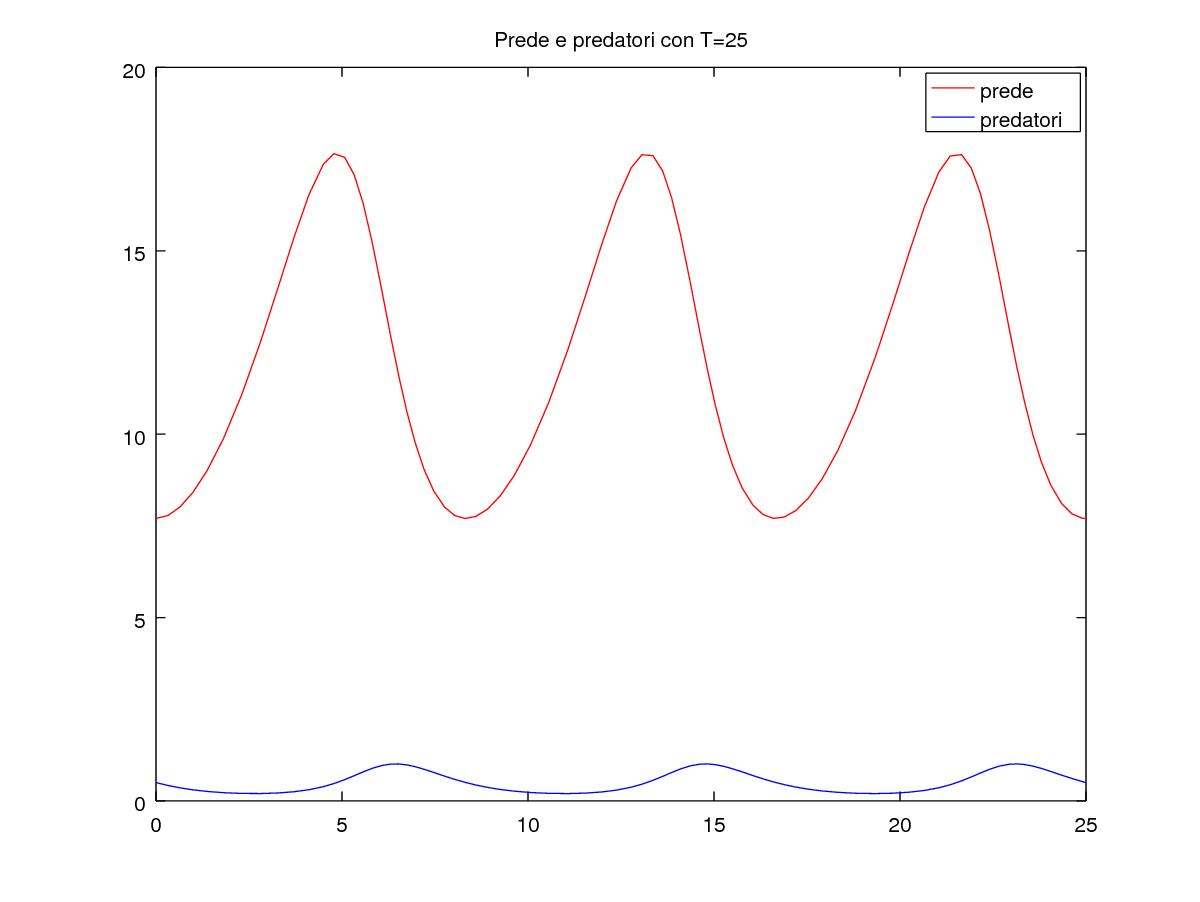
\includegraphics[width=\textwidth]{figs/predatori_prede_25.jpg}
\caption{Numero di prede e di predatori con T=25.}
\end{figure}
\end{center}

\newpage
\section{Esercizio 4}
L'equazione differenziale che risolve il problema è:

\[
I'(t) = r\cdot I(t)\cdot (N-I(t))
\]
Per risolvere il problema usiamo quindi lo script \emph{odefun4.m}:
\begin{lstlisting}[frame = trBL]
f=@(t, I) (0.0001*I(1)*(1000-I(1)));
[t, u] = ode45(f, [0, 100], 1);
i=min(find(u>=800));
t(i)
\end{lstlisting}
che ci da come risposta
\begin{lstlisting}[frame = lines]
>>odefun4

ans = 

   85.042
\end{lstlisting}

%QUARTO CAPITOLO
\chapter{Lezione IV}
\section{Esercitazione V}
\subsection{Esercizio 1}
Per risolvere l'esercizio 1 usiamo lo script \emph{ese1.m}:
\begin{lstlisting}[frame=trBL]
y0=[1200, 0];function [x,u] = RK4(odefun,tspan,y0,h)
% Risolve sull'intervallo [tspan(1),tspan(2)] il problema 
% a valori iniziali:
%   y'(x) = odefun(x,y(x))
%   y(tspan(1)) = y0
% usando il metodo di Runge-Kutta classico
%
% Dati di INPUT:
%   odefun    funzione da integrare inizializzata VETTORIALMENTE
%   tspan     intervallo di integrazione
%   y0        condizione iniziale PER COLONNA
%   h         passo di discretizzazione
%
% Dati di OUTPUT:
%   x       nodi equispaziati della griglia
%   u       soluzione numerica in corrispondenza dei nodi

x = [tspan(1):h:tspan(2)];
N = length(x);
ord=length(y0);
u = zeros(ord,N);  
u(:,1) = y0;
for i = 2:N
    f(:,1) = odefun(x(i-1),u(:,i-1));
    f(:,2) = odefun(x(i-1)+h/2,u(:,i-1)+h*f(:,1)/2);
    f(:,3) = odefun(x(i-1)+h/2, u(:,i-1)+h*f(:,2)/2);
    f(:,4) = odefun(x(i-1)+h, u(:,i-1)+h*f(:,3));
    u(:,i) = u(:,i-1)+h/6*(f(:,1)+2*f(:,2)+2*f(:,3)+f(:,4));
end
end


tslot=[0, 15];
h=0.01;
[x,y]=RK4(@f, tslot, y0, h);
y1=[y(1,1501), y(2,1501)];
tslot1=[15,147];
[t,u]=RK4(@f2, tslot1, y1, h); 
subplot(2,1,1)
plot(x, y(1, :), 'r')
hold on
plot(t, u(1,:), 'b')
legend('p. chiuso', 'p. aperto')
subplot(2,1,2)
plot(x, y(2, :), 'r')
hold on
plot(t,u(2,:),'b')
legend('p. chiuso', 'p. aperto')
\end{lstlisting}
dove \emph{f} è;
\begin{lstlisting}[frame=trbl]
function yp = f(x,y)
    yp = zeros(2,1);
    yp(1) = y(2);
    yp(2) = -16.4/90*y(2)-9.8;
end
\end{lstlisting}
ed \emph{f2} è:
\begin{lstlisting}[frame=trbl]
function yp = f2(x,y)
    yp = zeros(2,1);
    yp(1) = y(2);
    yp(2) = -180/90*y(2)-9.8;
end
\end{lstlisting}
dal quale otteniamo la seguente immagine:

\begin{center}
\begin{figure}[h!]
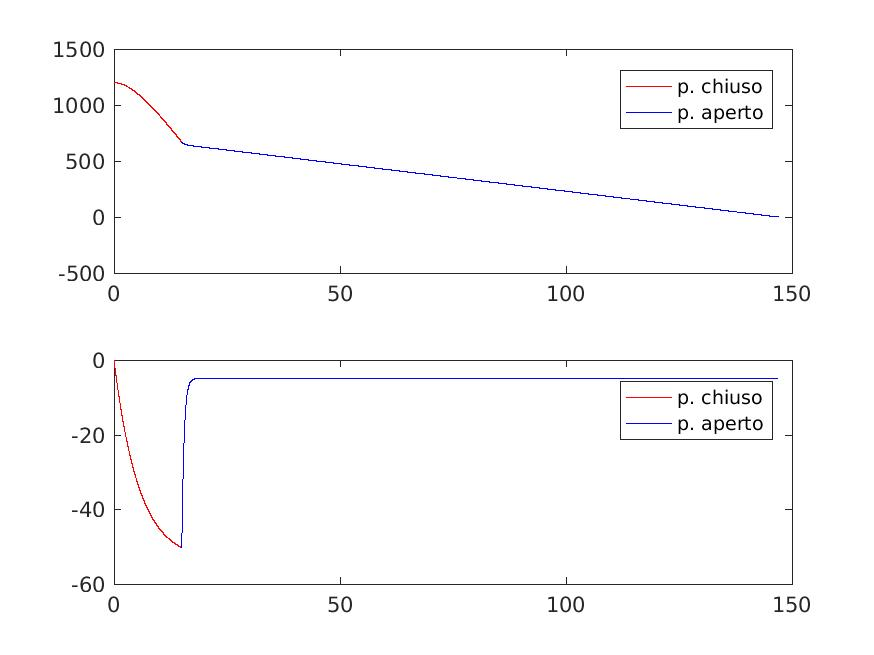
\includegraphics[width=\textwidth]{figs/ese1.jpg}
\caption{Spostamento e velocità del paracadutista.}
\end{figure}
\end{center}
\newpage
Osserviamo che $x_{max}$ è circa 147.

\subsection{Esercizio 2}
Per risolvere l'esercizio 2 usiamo lo script \emph{ese2.m}:
\begin{lstlisting}[frame=trBL]
y0=[pi/6, 0];
tslot=[0,10];
[x,y]=ode45(@f3, tslot, y0);
plot(x,y(:,1), 'r')
hold on
plot(x,y(:,2),'b')
legend('spostamento', 'velocita')
\end{lstlisting}
dove \emph{f3} è:
\begin{lstlisting}[frame=trbl]
function yp = f3(x,y)
    yp = zeros(2,1);
    yp(1) = y(2);
    yp(2) = -9.8/2*sin(y(1));
end
\end{lstlisting}
Otteniamo la seguente immagine:
\begin{center}
\begin{figure}[h!]
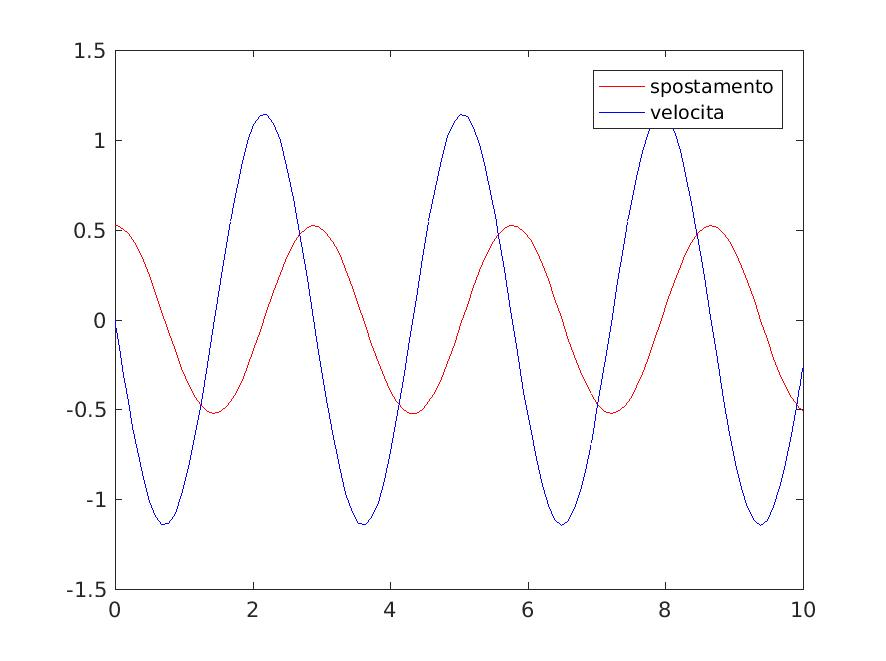
\includegraphics[width=\textwidth]{figs/ese2.jpg}
\caption{Spostamento e velocità del pendolo.}
\end{figure}
\end{center}

\subsection{Esercizio 3}
Lo script \emph{ese3.m} è:
\begin{lstlisting}[frame=trBL]
y0=[pi/6, 0];
tslot=[0,10];
[x,y]=ode45(@f4, tslot, y0);
plot(x,y(:,1), 'r')
hold on
plot(x,y(:,2),'b')
legend('spostamento', 'velocita')
\end{lstlisting}
dove \emph{f4} è:
\begin{lstlisting}[frame=trbl]
function yp = f4(x,y)
    yp = zeros(2,1);
    yp(1) = y(2);
    yp(2) = -9.8/2*y(1);
end
\end{lstlisting}
Otteniamo quindi la seguente immagine:
\begin{center}
\begin{figure}[h!]
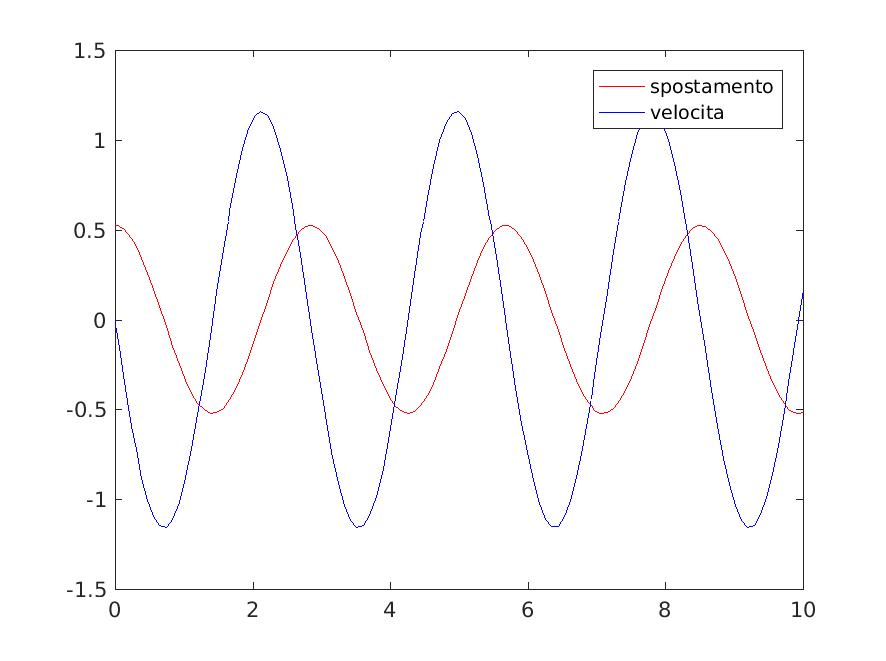
\includegraphics[width=\textwidth]{figs/ese3.jpg}
\caption{Spostamento e velocità del pendolo.}
\end{figure}
\end{center}

\newpage
\subsection{Esercizio 4}
Lo script \emph{ese4.m} è:
\begin{lstlisting}[frame=trBL]
scelta = menu('Scegli un oscillatore.',' Libero non Smorzato', ...
         'Libero Sottosmorzato', 'Libero Sovrasmorzato',...
         'Forzato Smorzato');
    
switch(scelta)
    case 1
        m=1; h=10; k=0; f=0; y0=[1; 0];
        titolo='Libero non Smorzato';
        name='libero_non_smorzato.jpg';
    case 2
        m=1; h=10; k=0.5; f=0; y0=[1; 0];
        titolo='Libero Sottosmorzato';
        name='libero_sottosmorzato.jpg';
    case 3
        m=1; h=10; k=10; f=0; y0=[1; 0];
        titolo='Libero Sovrasmorzato';
        name='libero_sovrasmorzato.jpg';
    case 4
        m=2; h=15; k=0.75; f=25; y0=[2; 0];
        titolo='Forzato Smorzato';
        name='forzato_smorzato.jpg';
end
        
f=@(x,y) [y(2); (-h*y(1)-k*y(2)+f)/m];
[x,u]=ode45(f, [0, 60], y0);

hold off
clear plot
hold on
plot(x,u(:,1),'r')
plot(x,u(:,2),'b')
legend('posizione','velocita')
xlabel('tempo')
title(titolo)
print(name,'-djpeg')
\end{lstlisting}
dal quale otteniamo il seguente menù:
\begin{center}
\begin{figure}[h!]
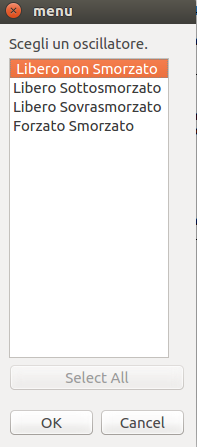
\includegraphics[width=0.3\textwidth]{figs/menu.png}
\caption{Menù esercizio 4.}
\end{figure}
\end{center}
\newpage
Cliccando sulle 4 opzioni si ottengono le seguenti 4 immagini:
\begin{figure}[h!]
\centering
\subfloat[][\emph{Libero non Smorzato}]
{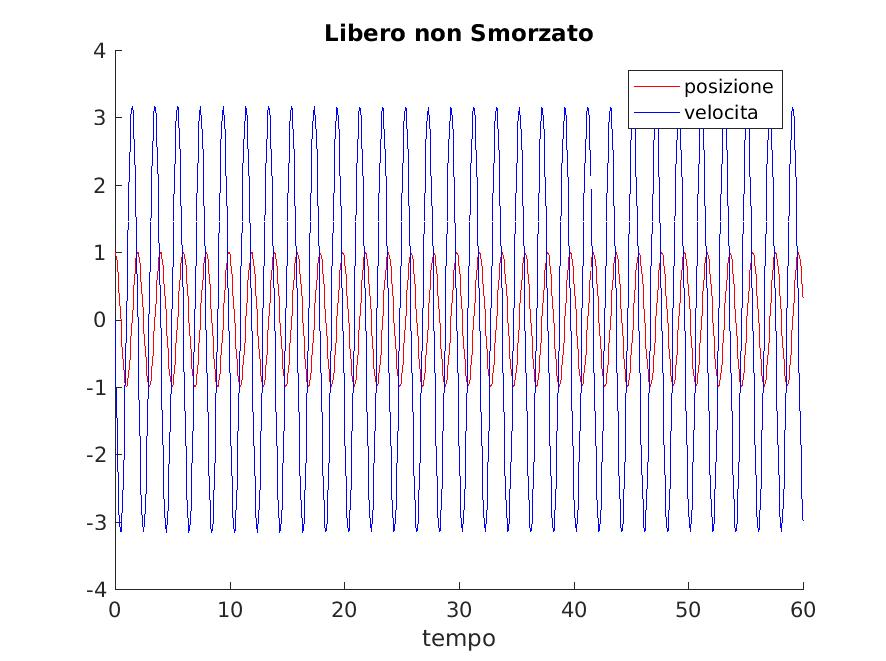
\includegraphics[width=.48\textwidth]{figs/libero_non_smorzato.jpg}} \quad
\subfloat[][\emph{Libero sottosmorzato}]
{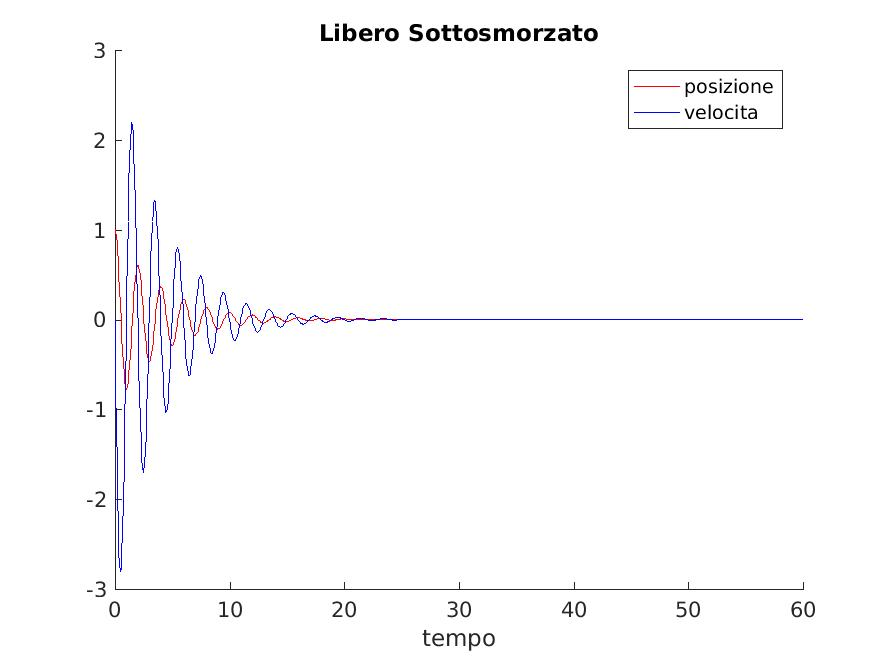
\includegraphics[width=.48\textwidth]{figs/libero_sottosmorzato.jpg}} \\
\subfloat[][\emph{Libero sovrasmorzato}]
{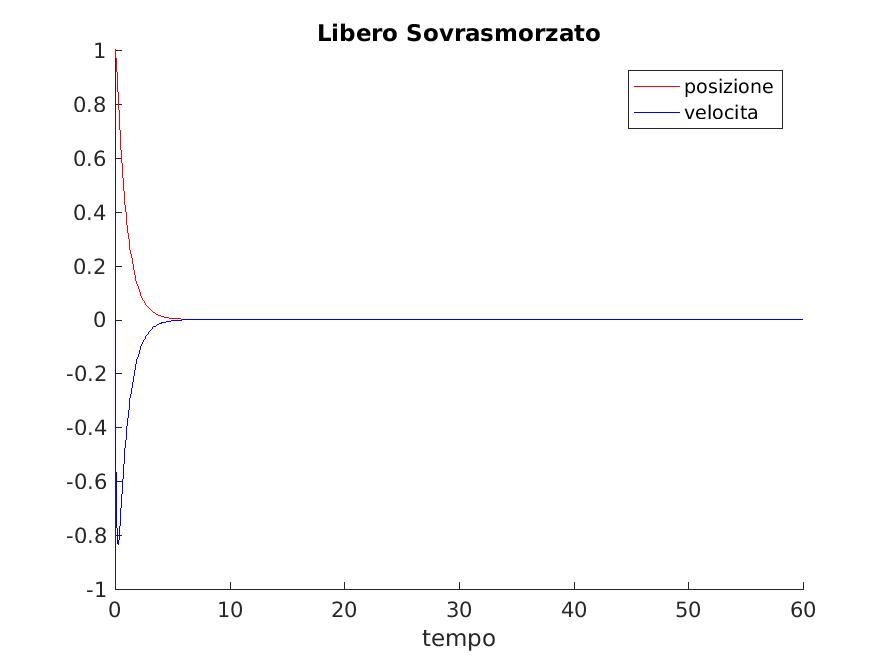
\includegraphics[width=.48\textwidth]{figs/libero_sovrasmorzato.jpg}} \quad
\subfloat[][\emph{Forzato smorzato}]
{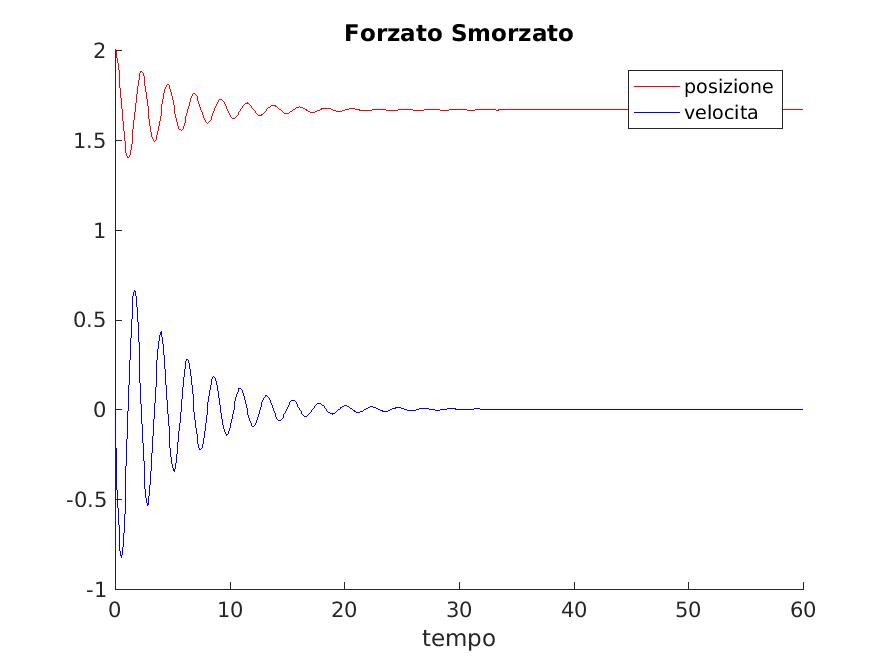
\includegraphics[width=.48\textwidth]{figs/forzato_smorzato.jpg}}
\caption{Immagini ottenute dall'esercizio 4.}
\end{figure}


\section{Esercitazione VI}
\subsection{Esercizio 1}
Per risolvere l'esercizio 1, usiamo lo script \emph{esercizio1.m}:
\begin{lstlisting}[frame = trBL]
g = 9.81;
m=1;
F = [0, 0, -g*m];
span = [0, 10];
init = [0, 1, 0, 0.8, 0, 1.2];
h = [0.0025, 0.00025, 0.005, 0.0005];

%la funzione per risolvere il sistema differenziale
f = @(t, y) [y(4);...
             y(5);...
             y(6);...
             1/m*(-(m*2*(y(4)^2+y(5)^2+y(6)^2) ...
             -2*y(3)*g*m)/(4*(y(1)^2 + y(2)^2 + y(3)^2))*2*y(1));
             1/m*(-(m*2*(y(4)^2 + y(5)^2 + y(6)^2) ...
             - 2*y(3)*g*m)/(4*(y(1)^2 + y(2)^2 + y(3)^2))*2*y(2));
             1/m*(-m*g-(m*2*(y(4)^2 + y(5)^2 + y(6)^2) ...
             - 2*y(3)*g*m)/(4*(y(1)^2 + y(2)^2 + y(3)^2))*2*y(3))];

%metodo di Eulero con h=0.0025 e h=0.00025             
[t, u] = eulero_esplicito(f, span, init, h(1));
max_residuo = max(abs(u(:,1).^2 + u(:,2).^2 + u(:,3).^2-1))

[t, u] = eulero_esplicito(f, span, init, h(2));
max_residuo = max(abs(u(:,1).^2 + u(:,2).^2 + u(:,3).^2-1))

%metodo di Runge_Kutta con h=0.005 e h=0.0005
[t, u] = RK4(f, span, init, h(3));
max_residuo = max(abs(u(1, :).^2 + u(2, :).^2 + u(3, :).^2-1))

[t, u] = RK4(f, span, init, h(3));
max_residuo = max(abs(u(1, :).^2 + u(2, :).^2 + u(3, :).^2-1))
plot3(u(1, :), u(2, :), u(3, :));

%funzione ode23
[t, u] = ode23(f, span, init);
max_residuo = max(abs(u(:, 1).^2 + u(:, 2).^2 + u(:, 3).^2-1))

%funzione ode45 con diversi valori di Reltol
reltol = [0.001,0.0001,0.00001];

[x, u] = ode45(f, span, init, odeset('RelTol', reltol(1)));
max_residuo = max(abs(u(:, 1).^2 + u(:, 2).^2 + u(:, 3).^2-1))

[x, u] = ode45(f, span, init, odeset('RelTol', reltol(2)));
max_residuo = max(abs(u(:, 1).^2 + u(:, 2).^2 + u(:, 3).^2-1))

[x, u] = ode45(f, span, init, odeset('RelTol', reltol(3)));
max_residuo = max(abs(u(:, 1).^2 + u(:, 2).^2 + u(:, 3).^2-1))
\end{lstlisting}
dal quale otteniamo come risultati:
\begin{lstlisting}[frame = lines]
>> esercizio1
max_residuo =  0.44821
max_residuo =  0.043519
max_residuo =    4.8131e-06
max_residuo =    4.8131e-06
max_residuo =    4.8827e-06
max_residuo =  0.061113
max_residuo =  0.0091891
max_residuo =    6.6768e-04
\end{lstlisting}
che indicano rispettivamente i residui massimi del metodo di Eulero con 
h = 0.0025 e h=0.00025, del metodo di Runge-Kutta con h = 0.005 e h = 0.0005,
del risultato ottenuto con la funzione ode23 e dei risultati ottenuti con la 
funzione ode45 usata con i valori di RelTol = 0.001, 0.0001, 0.00001.
\par
La funzione \emph{eulero\_esplicito} è ottenuta modificando la funzione 
\emph{eulero}:
\begin{lstlisting}[frame = trBL]
function [x,u] = eulero_esplicito(odefun,slot,init,h)

x=[slot(1):h:slot(2)];
N=length(x);
u = zeros(N, length(init));  
u(1, :) = init;
for i = 2:N
    ff = odefun(x(i-1),u(i-1, :))';
    u(i, :) = u(i-1, :)+h*ff;
end

end
\end{lstlisting}
%\newpage
Il plot della traiettoria del punto $z$, ottenuto con \emph{plot3}, è:
\begin{center}
\begin{figure}[h!]
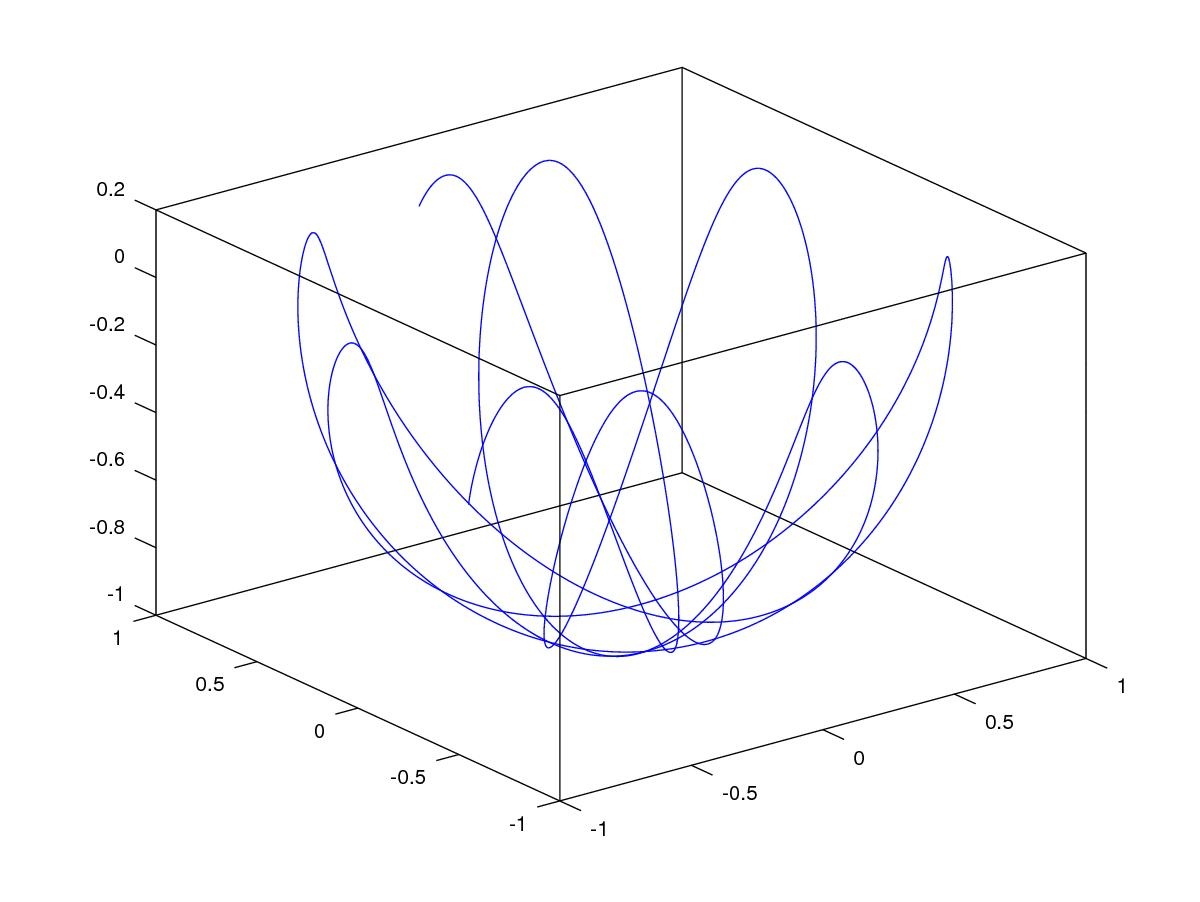
\includegraphics[width=0.5\textwidth]{figs/esercizio1.jpg}
\caption{Traiettoria del punto $z$.}
\end{figure}
\end{center}

\subsection{Esercizio 2}
Risolviamo questo esercizio con lo script \emph{esercizio2.m}:
\begin{lstlisting}[frame = trBL]
s = 10;
r = 28;
b = 8/3;
init1 = [10, 0, 20];
init2 = [11, 0, 20];
xmax = 30;

%funzione di Lorenz
f=@(t, y) [s*(y(2)-y(1)); r*y(1)-y(2)-y(1)*y(3); y(1)*y(2)-b*y(3)];

%risolviamo con i valori iniziali init1
[t, y] = ode45(f, [0, xmax], init1);
figure;
subplot(3, 1, 1);
plot(t, y(:, 1));
legend('y1');
subplot(3, 1, 2);
plot(t, y(:, 2));
legend('y2');
subplot(3, 1, 3);
plot(t, y(:, 3));
legend('y3');

figure;
plot3(y(:,1), y(:,2), y(:,3));
title('y1, y2, y3');

%risolviamo con i valori iniziali init2
[t, y] = ode45(f, [0, xmax], init2);
figure;
subplot(3, 1, 1);
plot(t, y(:, 1));
legend('y1');
subplot(3, 1, 2);
plot(t, y(:, 2));
legend('y2');
subplot(3, 1, 3);
plot(t, y(:, 3));
legend('y3');

figure;
plot3(y(:,1), y(:,2), y(:,3));
title('y1, y2, y3');
\end{lstlisting}
Le immagini ottenute da questo script sono:
\begin{center}
\begin{figure}[h!]
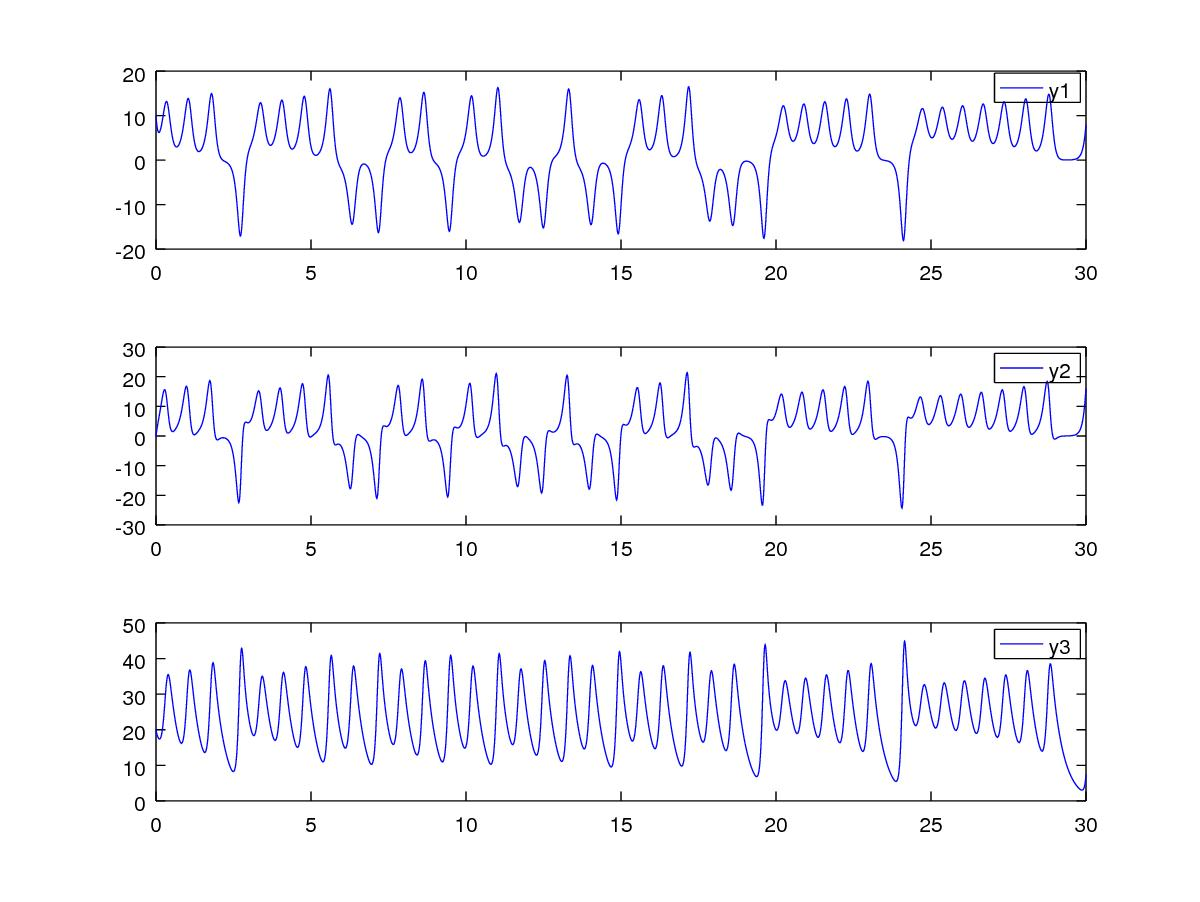
\includegraphics[width=\textwidth]{figs/esercizio2_1.jpg}
\caption{Grafici di $(x, y1), (x, y2), (x, y3)$.}
\end{figure}
\end{center}

\begin{center}
\begin{figure}[h!]
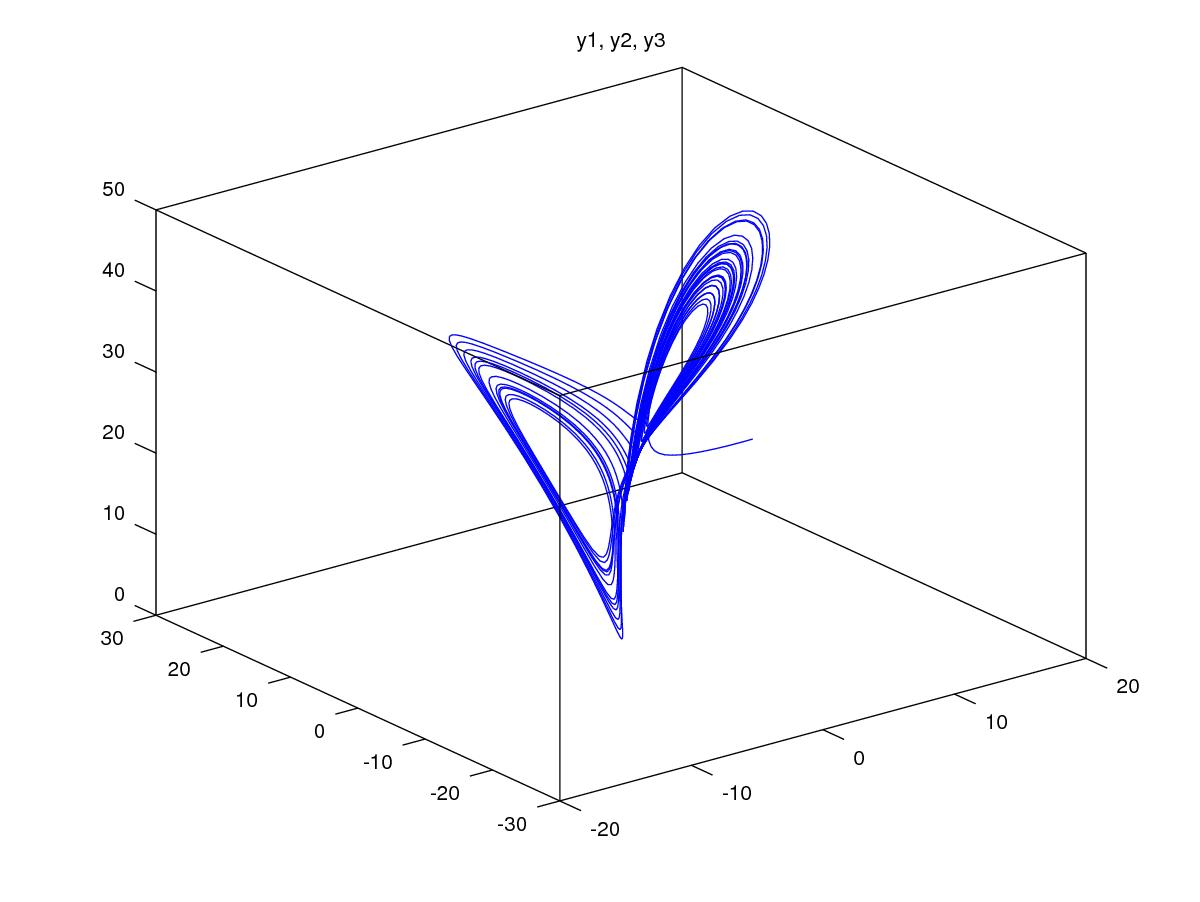
\includegraphics[width=\textwidth]{figs/esercizio2_2.jpg}
\caption{Grafico di $(y1, y2, y3)$.}
\end{figure}
\end{center}

\begin{center}
\begin{figure}[h!]
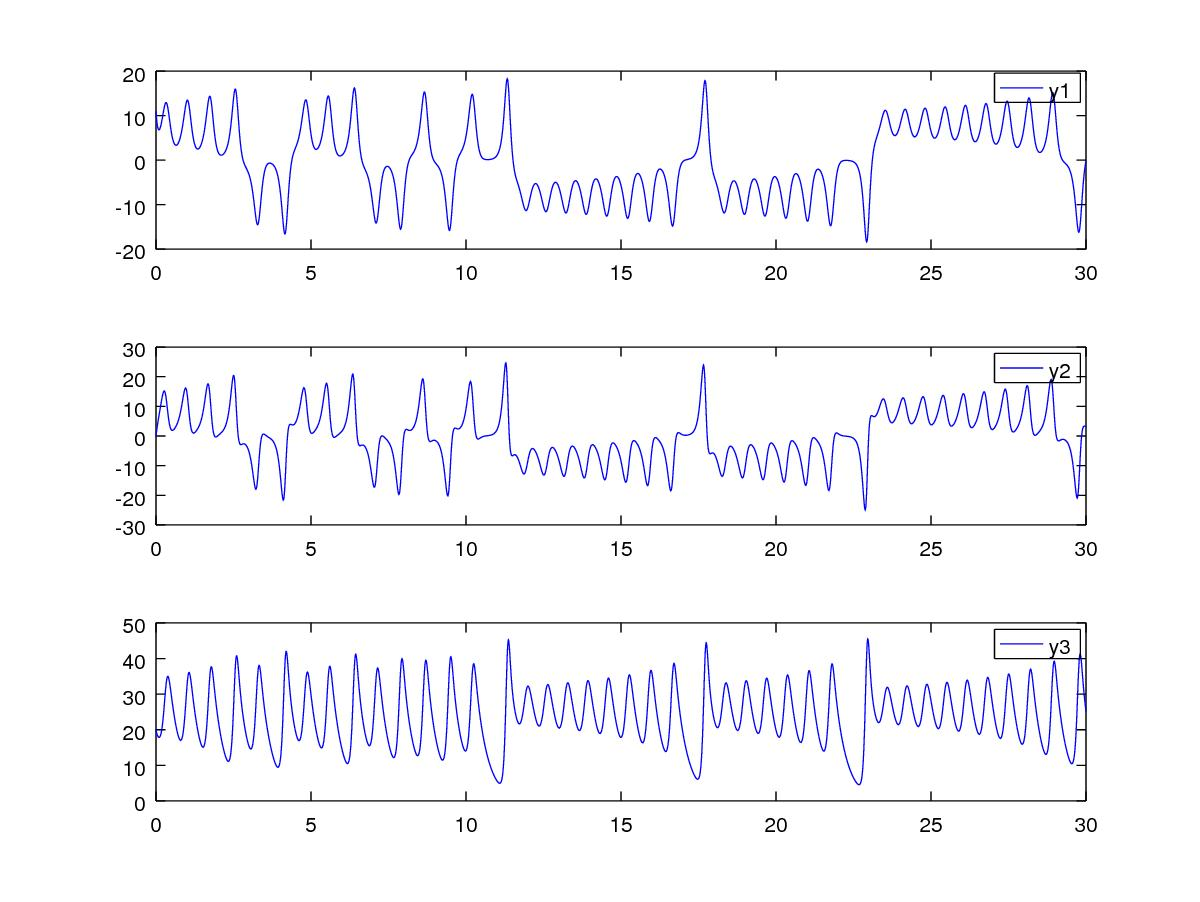
\includegraphics[width=\textwidth]{figs/esercizio2_3.jpg}
\caption{Grafici di $(x, y1), (x, y2), (x, y3)$.}
\end{figure}
\end{center}

\begin{center}
\begin{figure}[h!]
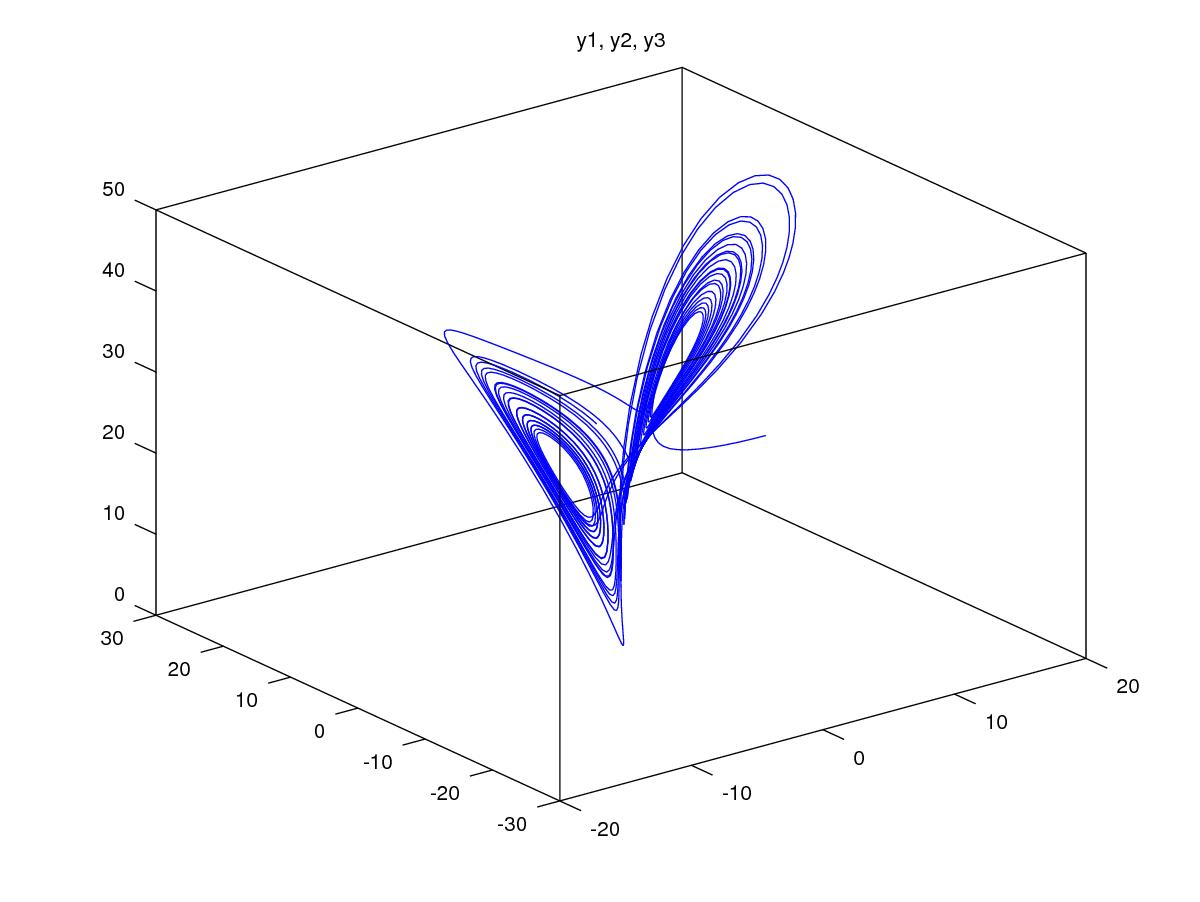
\includegraphics[width=\textwidth]{figs/esercizio2_4.jpg}
\caption{Grafico di $(y1, y2, y3)$.}
\end{figure}
\end{center}

\newpage
Osserviamo che anche per piccole variazioni dei dati iniziali, i grafici di 
$(x, y1), (x, y2), (x, y3)$ sono molto diversi.

\newpage
\subsection{Esercizio 3}
Lo script \emph{esercizio3.m} è:
\begin{lstlisting}[frame = trBL]
mu = [0.1, 1, 10, 100];
slot = [0, 100];
init = [1, 1];

for i=1:4
    f=@(t, y) [y(2); mu(i)*(1-y(1).^2).*y(2)-y(1)];
    
    [t1, y1]=ode45(f, slot, init);
    [t2, y2]=ode15s(f, slot, init);
    [t3, y3]=eulero_esplicito(f, slot, init, 0.01);
    
    figure;
    subplot(2, 3, 1)
    plot(t1, y1(:, 1), 'r');
    legend('ode45');
    subplot(2, 3, 2)
    plot(t2, y2(:, 1), 'r');
    legend('ode15s');
    subplot(2, 3, 3)
    plot(t3, y3(:, 1), 'r');
    legend('eulero_esplicito');
    subplot(2, 3, 4)
    plot(y1(:, 1),y1(:,2) ,'r');
    legend('ode45');
    subplot(2, 3, 5)
    plot(y2(:, 1),y2(:,2) ,'r');
    legend('ode15s');
    subplot(2, 3, 6)
    plot(y3(:, 1),y3(:,2) ,'r');
    legend('eulero_esplicito');
    
    length(t1)
    length(t2)
    length(t3)

end
\end{lstlisting}
dal quale si ottengono le seguenti immagini:
\begin{center}
\begin{figure}[h!]
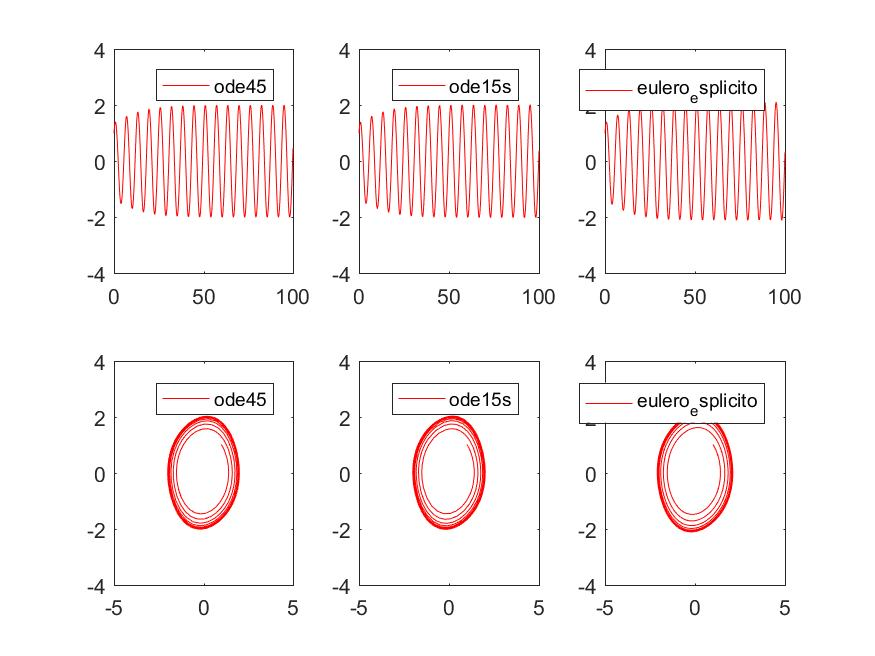
\includegraphics[width=\textwidth]{figs/esercizio3_1.jpg}
\caption{$\mu = 0.1$.}
\end{figure}
\end{center}

\begin{center}
\begin{figure}[h!]
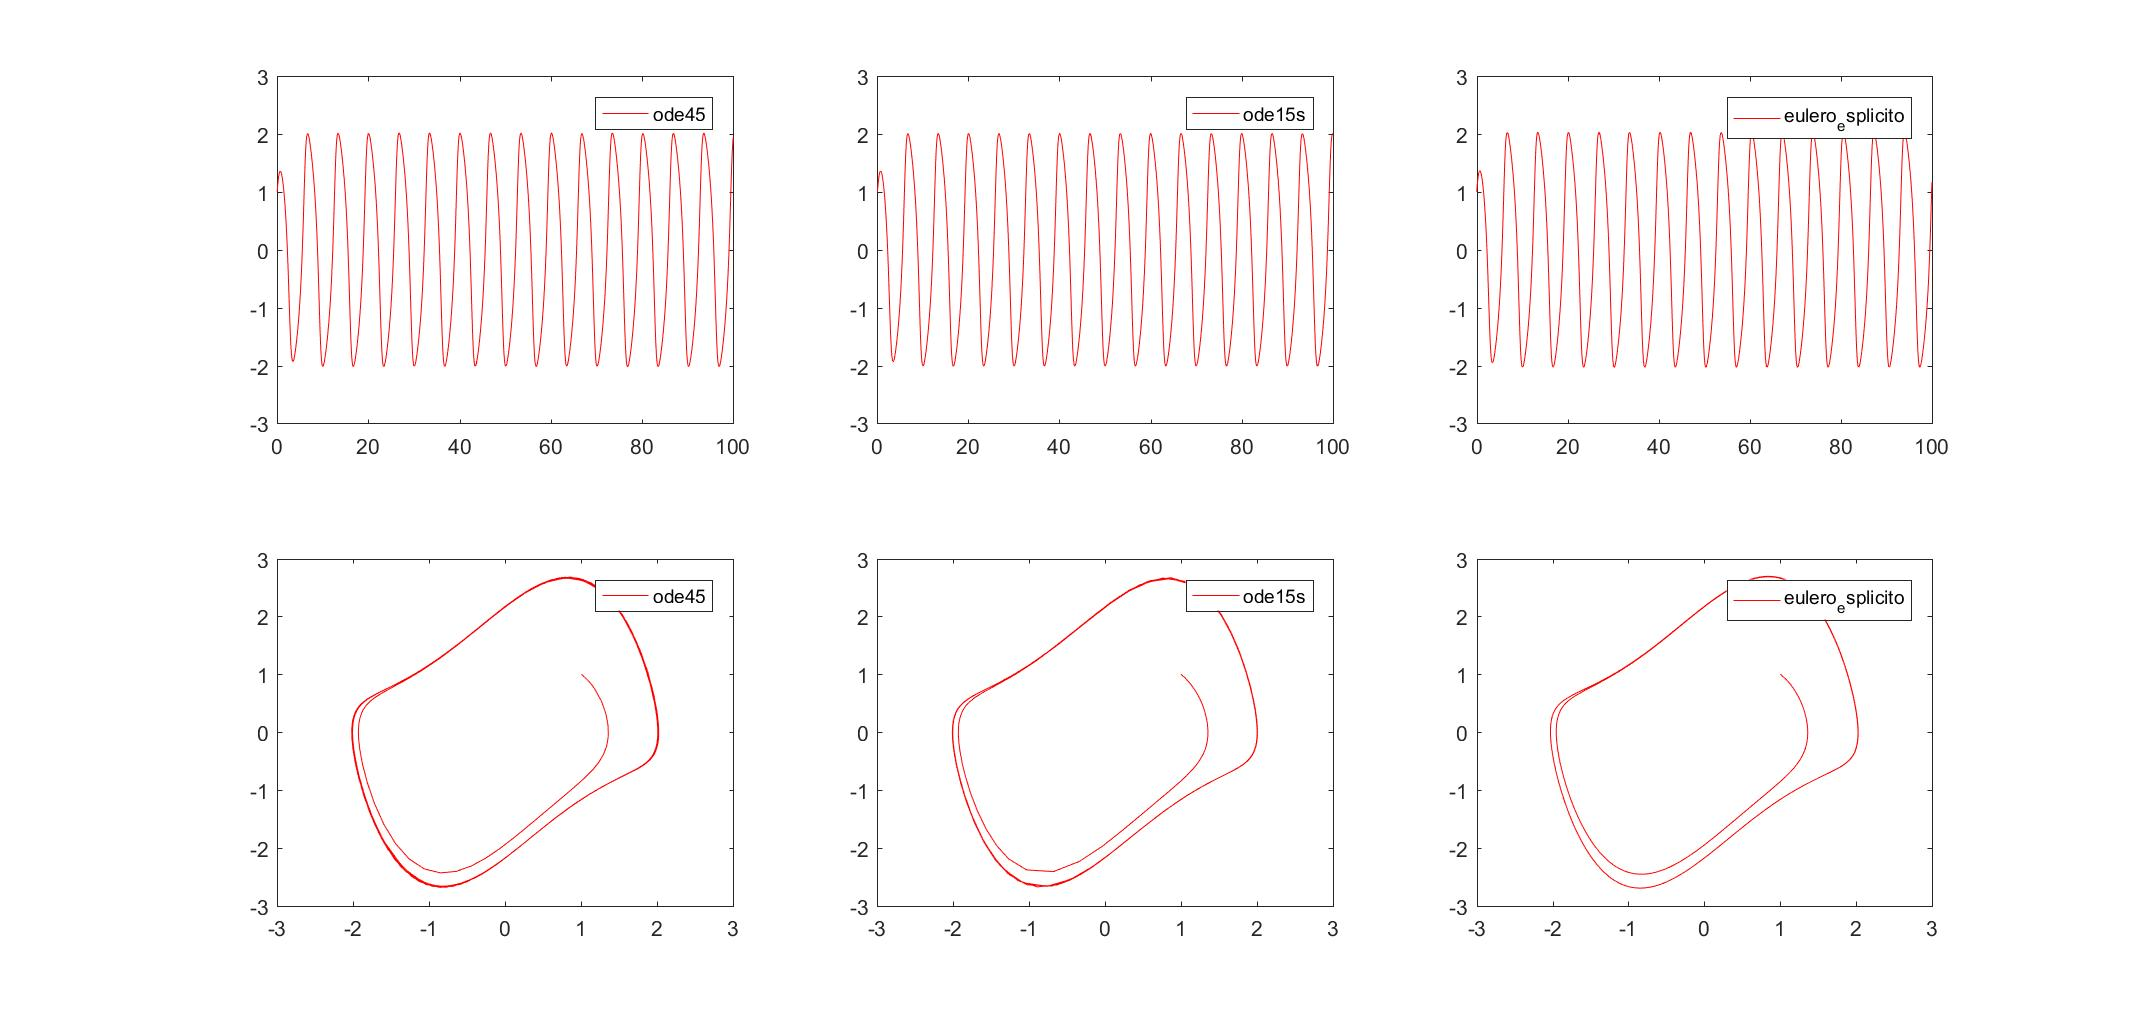
\includegraphics[width=\textwidth]{figs/esercizio3_2.jpg}
\caption{$\mu = 1$.}
\end{figure}
\end{center}

\begin{center}
\begin{figure}[h!]
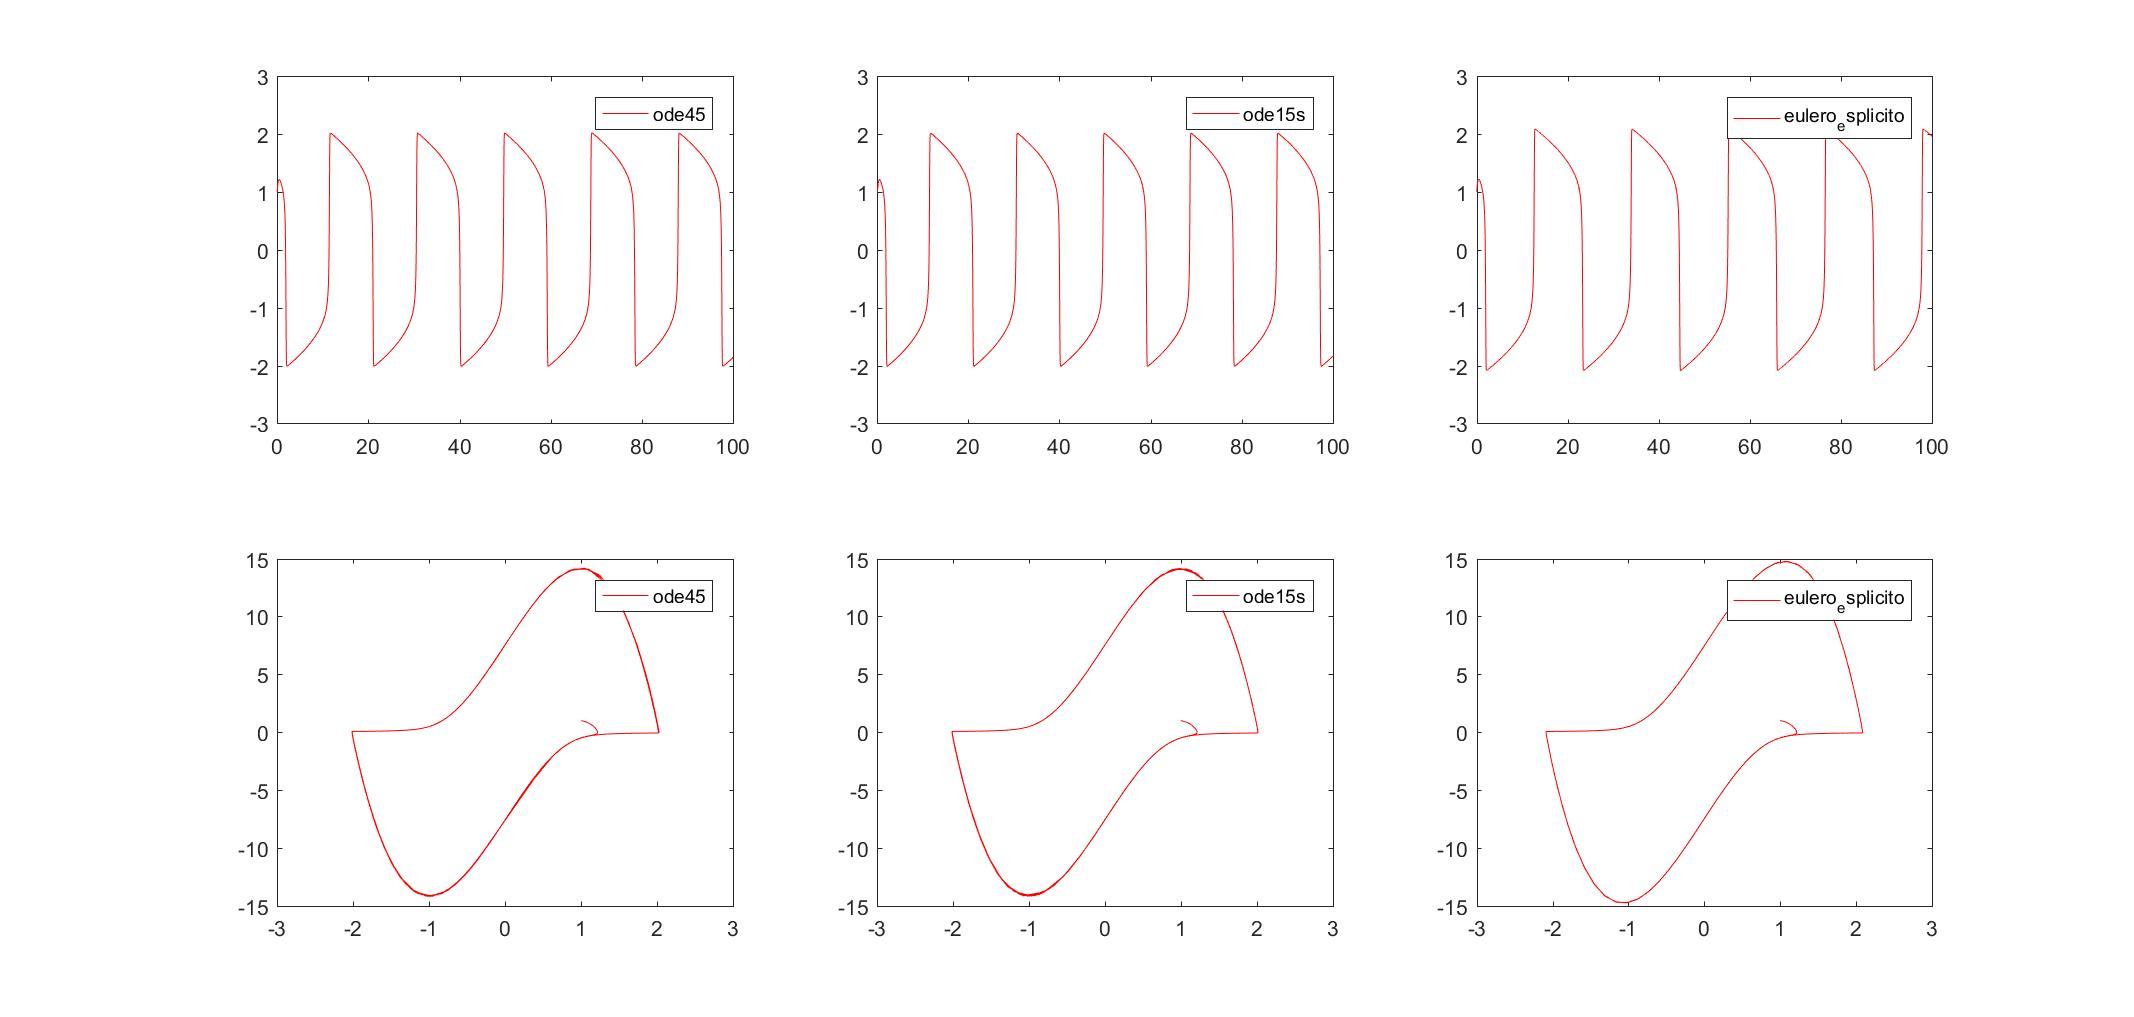
\includegraphics[width=\textwidth]{figs/esercizio3_3.jpg}
\caption{$\mu = 10$.}
\end{figure}
\end{center}

\begin{center}
\begin{figure}[t!]
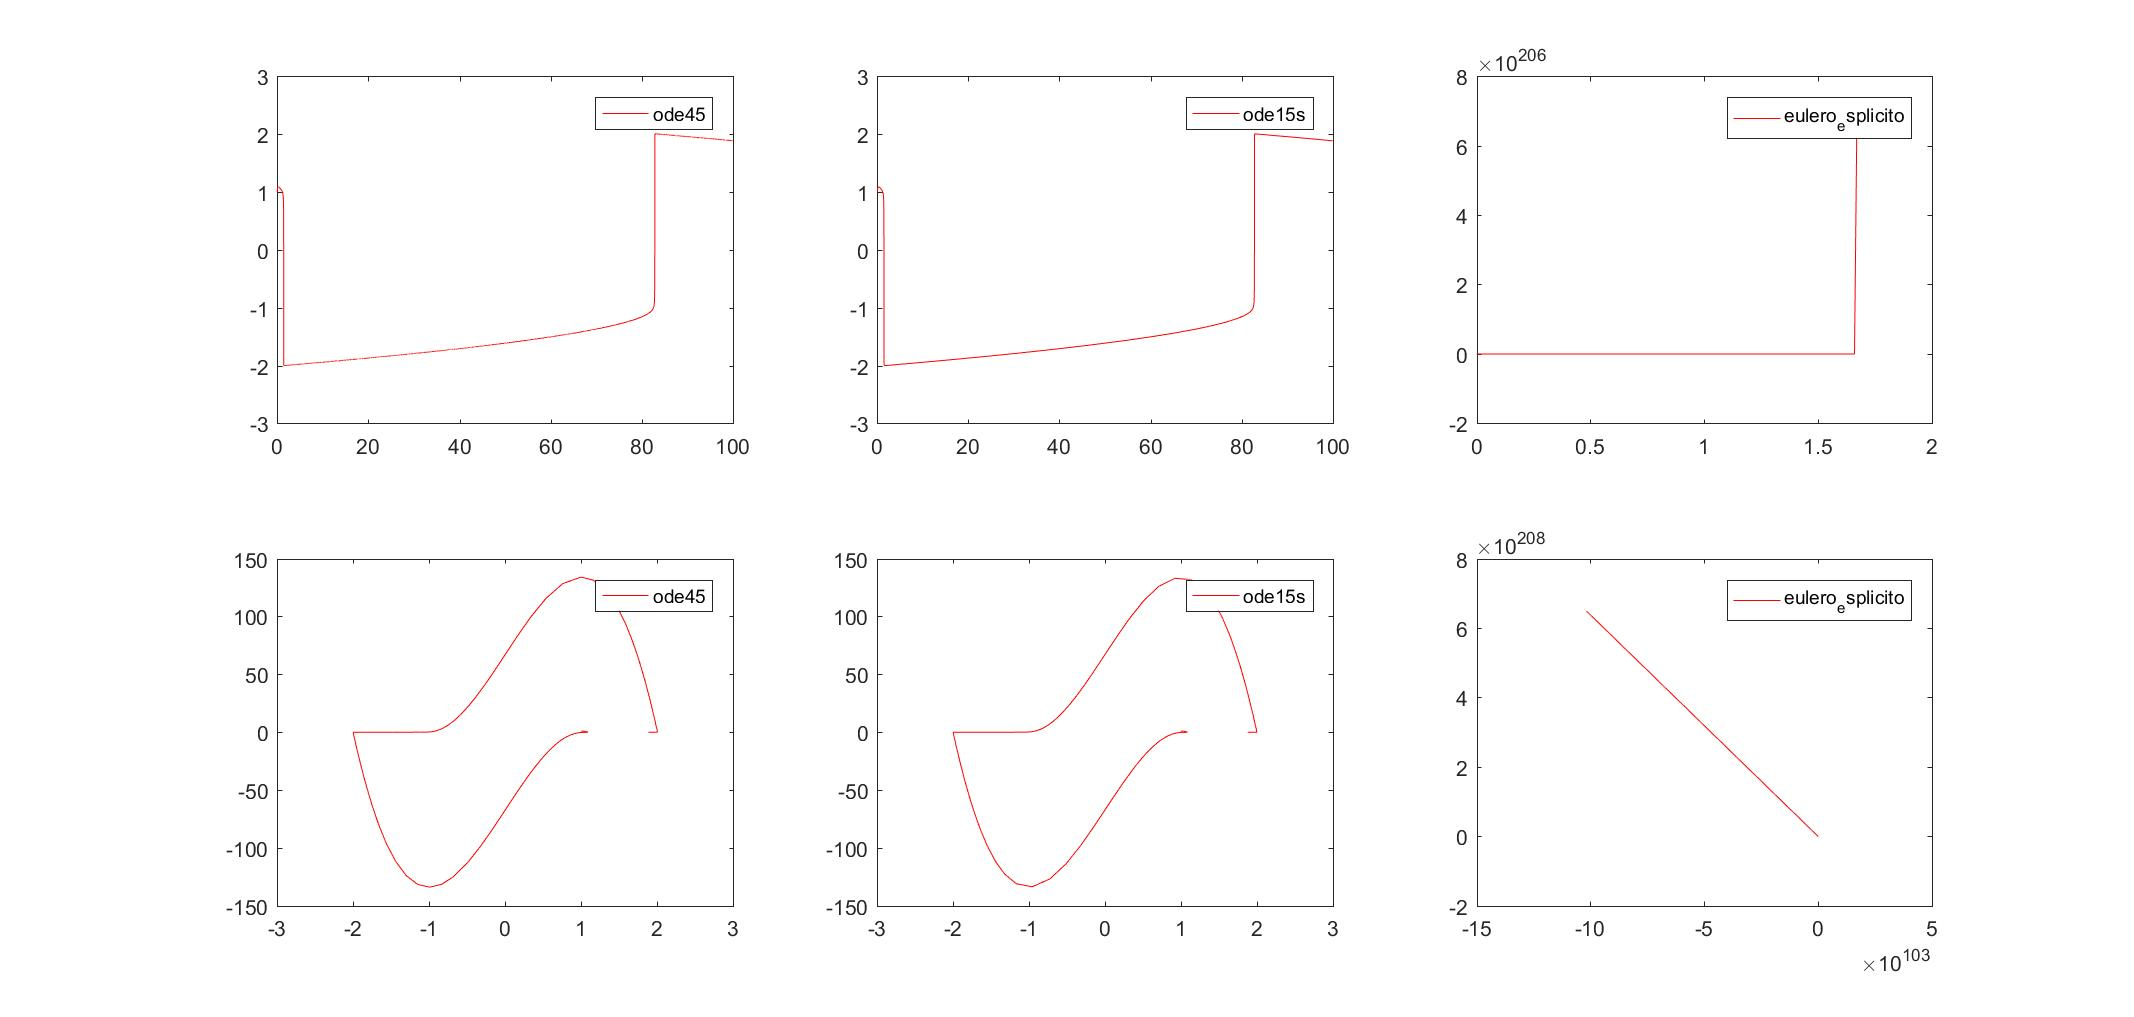
\includegraphics[width=\textwidth]{figs/esercizio3_4.jpg}
\caption{$\mu = 100$.}
\end{figure}
\end{center}

\newpage
Si osserva che il metodo di Eulero fallisce per valori grandi di $\mu$, nella fattispecie
per $\mu=100$.

%QUINTO CAPITOLO
\chapter{Lezione V}
\section{Esercitazione VII}
\subsection{Esercizio 1}
Per risolvere l'esercizio 1 usiamo lo script \emph{ese\_1.m}:
\begin{lstlisting}[frame = trBL]
f1=@(x,y) [cos(x.^2); sin(x.^2)]
y0=[0;0];
[x1,y1]=ode45(f1,[-10,10],y0);
plot3(x1,y1(:,1),y1(:,2),'b')
\end{lstlisting}
dal quale si ottiene la seguente immagine:
\begin{center}
\begin{figure}[h!]
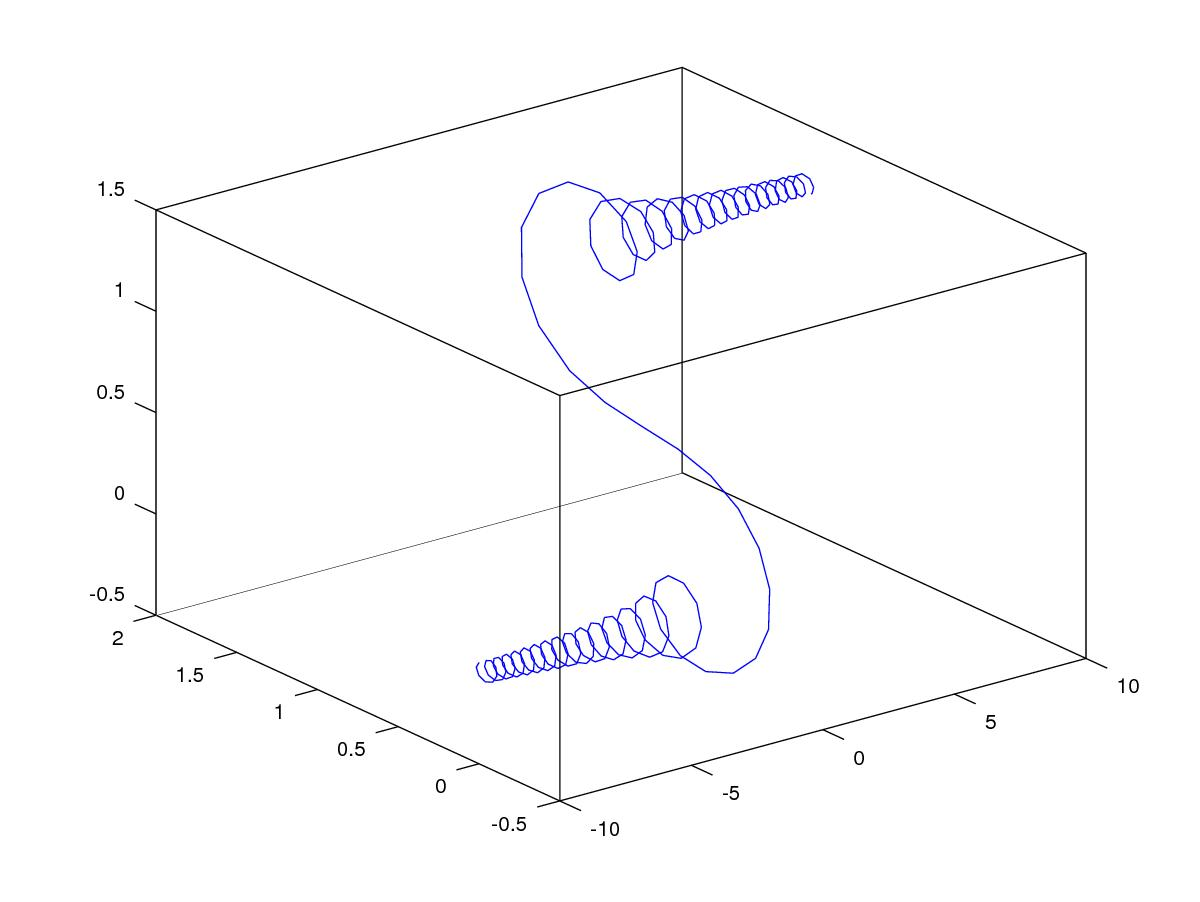
\includegraphics[width=\textwidth]{figs/spirali.jpg}
\caption{Spirale di Cornu.}
\end{figure}
\end{center}


\newpage
\subsection{Esercizio 2}
Per risolvere l'esercizio 2, usiamo lo script \emph{ese\_2.m}:
\begin{lstlisting}[frame = trBL]
% Imposto i parametri
b = 1.04;
a = 1;
estremo = 300;

xp=@(x,y)log(b)*x-y;
yp=@(x,y)log(b)*y+x;
xpp=@(x,y)((log(b))^2)*x-2*log(b)*y-x;
ypp=@(x,y)((log(b))^2)*y+2*log(b)*x-y;
curvatura=@(x,y)norm(xp(x,y)*ypp(x,y)-yp(x,y)*xpp(x,y))/...
               ((xp(x,y))^2+(yp(x,y))^2)^(3/2);

f = @(x, y) [cos(y(3));sin(y(3));curvatura(y(1),y(2))];

% Risolvo quindi la curva e ne faccio il grafico
[u, y] = ode45(f,[-estremo, estremo],[a;0;curvatura(a,0)]);
plot(y(:, 1), y(:, 2));
\end{lstlisting}
Lanciandolo si ottiene la seguente immagine:
\begin{center}
\begin{figure}[h!]
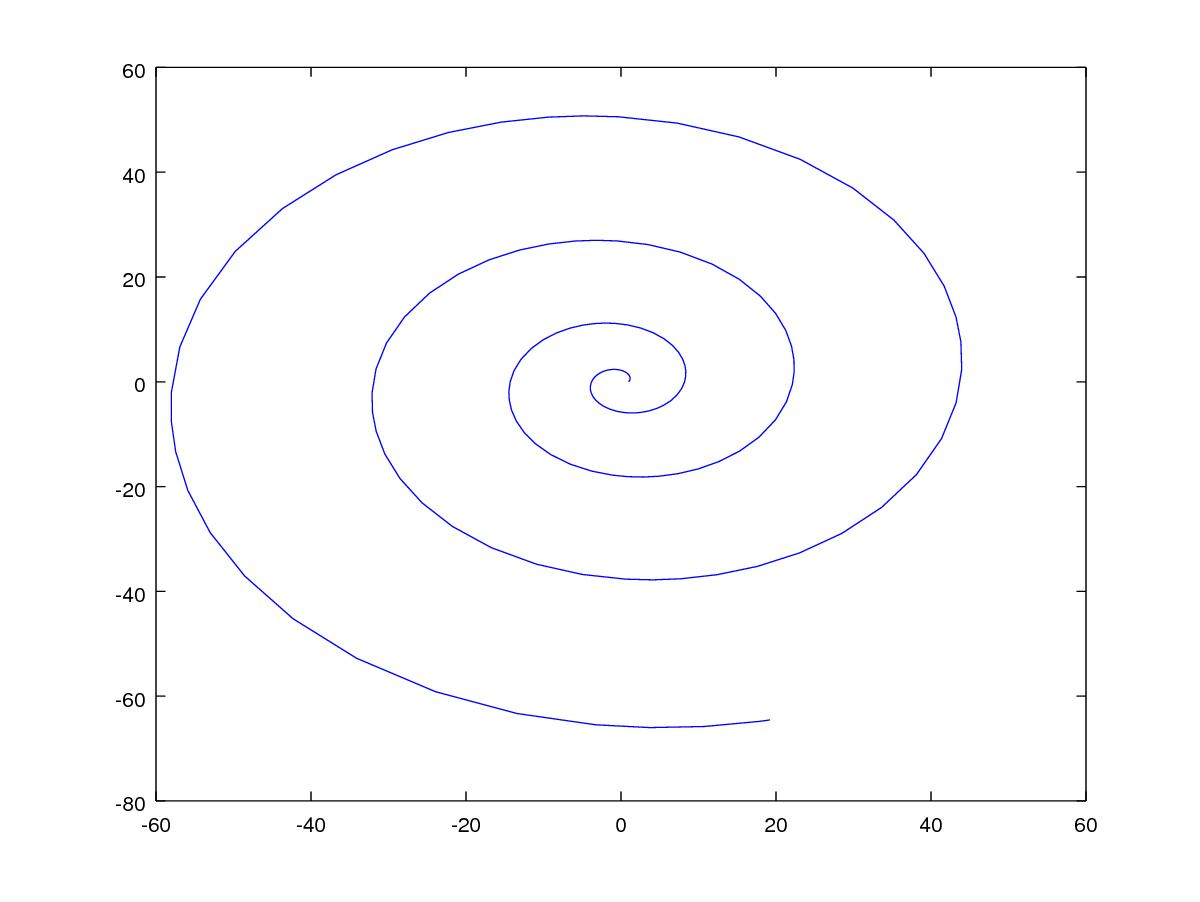
\includegraphics[width=\textwidth]{figs/spirale.jpg}
\caption{Spirale logaritmica.}
\end{figure}
\end{center}

\end{document}
